% ****************************************************************************************** % Dissertation template and document class for Princeton University
% Author  : Jeffrey Scott Dwoskin <jdwoskin@princeton.edu>
% Adapted from: http://www.math.princeton.edu/graduate/tex/puthesis.html
% ****************************************************************************************** %


%%% For print copies
%% set 'singlespace' option to set entire thesis to single space, and define "\printmode" to remove all hyperlinks for printed copies of the thesis. Delete all output files before changing this mode -- it will turn hyperref package on and off
%\documentclass[12pt,lot, lof, singlespace]{puthesis}
%\newcommand{\printmode}{}

%%% For the electronic copy, use doublespacing, define "\proquestmode" to use outlined links, instead of colored links. 
\documentclass[12pt,lot, lof]{puthesis}
%\newcommand{\proquestmode}{}
%\newcommand{\printmode}{}
% I prefer proquestmode to be off for electronic copies for normal use, since the colored links are less distracting. However when printed in black and white, the colored links are difficult to read. 

%%% For early drafts without some of the frontmatter
% Also see the "ifodd" command below to disable more frontmatter
%\documentclass[12pt]{puthesis}

%%%%%%%%%%%%%%%%%%%%%%%%%%%%%%%%%%%%%%%%%%%%%%%%%%%%%%%%%%%%%\
%%%% Author & title page info

\title{Methods for Materials Characterization in Batteries Using Acoustic Interrogation}

\submitted{September 2015}  % degree conferral date (January, April, June, September, or November)
\copyrightyear{2015}  % year in which the copyright is secured by publication of the dissertation.
\author{Shoham Bhadra}
\adviser{Daniel A. Steingart}  %replace with the full name of your adviser
%\departmentprefix{Program in}  % defaults to "Department of", but programs need to change this.
\department{Electrical Engineering}

%%%%%%%%%%%%%%%%%%%%%%%%%%%%%%%%%%%%%%%%%%%%%%%%%%%%%%%%%%%%%\
%%%% Tweak float placements
% From: http://mintaka.sdsu.edu/GF/bibliog/latex/floats.html "Controlling LaTeX Floats"
% and based on: http://www.tex.ac.uk/cgi-bin/texfaq2html?label=floats
% LaTeX defaults listed at: http://people.cs.uu.nl/piet/floats/node1.html

% Alter some LaTeX defaults for better treatment of figures:
    % See p.105 of "TeX Unbound" for suggested values.
    % See pp. 199-200 of Lamport's "LaTeX" book for details.
    %   General parameters, for ALL pages:
    \renewcommand{\topfraction}{0.85}	% max fraction of floats at top
    \renewcommand{\bottomfraction}{0.6}	% max fraction of floats at bottom
    %   Parameters for TEXT pages (not float pages):
    \setcounter{topnumber}{2}
    \setcounter{bottomnumber}{2}
    \setcounter{totalnumber}{4}     % 2 may work better
    \setcounter{dbltopnumber}{2}    % for 2-column pages
    \renewcommand{\dbltopfraction}{0.66}	% fit big float above 2-col. text
    \renewcommand{\textfraction}{0.15}	% allow minimal text w. figs
    %   Parameters for FLOAT pages (not text pages):
    \renewcommand{\floatpagefraction}{0.66}	% require fuller float pages
	% N.B.: floatpagefraction MUST be less than topfraction !!
    \renewcommand{\dblfloatpagefraction}{0.66}	% require fuller float pages

% The documentclass already sets parameters to make a high penalty for widows and orphans. 

%%%%%%%%%%%%%%%%%%%%%%%%%%%%%%%%%%%%%%%%%%%%%%%%%%%%%%%%%%%%%\
%%%% Use packages

%\usepackage{amsfonts}

%%% For figures
\usepackage{graphicx}
%\usepackage{subfig,rotate}

%%% for comments
\usepackage{verbatim}

%%% For tables
\usepackage{multirow}
% Longtable lets you have tables that span multiple pages.
\usepackage{longtable}

% Booktabs produces far nicer tables than the standard LaTeX tables.
%   see: http://en.wikibooks.org/wiki/LaTeX/Tables
\usepackage{booktabs}
\usepackage{tabularx}

\usepackage[version=3]{mhchem}
\usepackage{graphicx} 
% \usepackage{lastpage}
\usepackage[format=plain,justification=raggedright,singlelinecheck=false,font=small,labelfont=bf,labelsep=space]{caption} 
% \usepackage{stfloats}
% \usepackage{xcolor}
\usepackage{gensymb}
\usepackage{array}
\setlength\extrarowheight{4pt} 

%set parameters for longtable:
% default caption width is 4in for longtable, but wider for normal tables
\setlength{\LTcapwidth}{\textwidth}



%%%%%%%%%%%%%%%%%%%%%%%%%%%%%%%%%%%%%%%%%%%%%%%%%%%%%%%%%%
%%% Printed vs. online formatting
\ifdefined\printmode

% Printed copy
% url package understands urls (with proper line-breaks) without hyperlinking them
\usepackage{url}


\else

\ifdefined\proquestmode
%ProQuest copy -- http://www.princeton.edu/~mudd/thesis/Submissionguide.pdf

% ProQuest requires a double spaced version (set previously). They will take an electronic copy, so we want links in the pdf, but also copies may be printed or made into microfilm in black and white, so we want outlined links instead of colored links.
\usepackage{hyperref}
\hypersetup{bookmarksnumbered}
\setlength{\oddsidemargin}{0in}
\setlength{\evensidemargin}{0in}
\setlength{\topmargin}{-.5in}
\setlength{\textheight}{9.03in}
\setlength{\textwidth}{6.5in}
\setlength{\footskip}{0.2in}

% copy the already-set title and author to use in the pdf properties
\makeatletter
\hypersetup{pdftitle=\@title,pdfauthor=\@author}
\makeatother

\else
% Online copy

% adds internal linked references, pdf bookmarks, etc

% turn all references and citations into hyperlinks:
%  -- not for printed copies
% -- automatically includes url package
% options:
%   colorlinks makes links by coloring the text instead of putting a rectangle around the text.
\usepackage{hyperref}
\hypersetup{colorlinks,bookmarksnumbered,linkcolor = blue,
            urlcolor  = blue,
            citecolor = blue,
            anchorcolor = blue}

% copy the already-set title and author to use in the pdf properties
\makeatletter
\hypersetup{pdftitle=\@title,pdfauthor=\@author}
\makeatother

% make the page number rather than the text be the link for ToC entries
%\hypersetup{linktocpage}
\fi % proquest or online formatting
\fi % printed or online formatting


%%%%%%%%%%%%%%%%%%%%%%%%%%%%%%%%%%%%%%%%%%%%%%%%%%%%%%%%%%%%%\
%%%% Define commands

% Define any custom commands that you want to use.
% For example, highlight notes for future edits to the thesis
%\newcommand{\todo}[1]{\textbf{\emph{TODO:}#1}}


% create an environment that will indent text
% see: http://latex.computersci.org/Reference/ListEnvironments
% 	\raggedright makes them left aligned instead of justified
\newenvironment{indenttext}{
    \begin{list}{}{ \itemsep 0in \itemindent 0in
    \labelsep 0in \labelwidth 0in
    \listparindent 0in
    \topsep 0in \partopsep 0in \parskip 0in \parsep 0in
    \leftmargin 1em \rightmargin 0in
    \raggedright
    }
    \item
  }
  {\end{list}}

% another environment that's an indented list, with no spaces between items -- if we want multiple items/lines. Useful in tables. Use \item inside the environment.
% 	\raggedright makes them left aligned instead of justified
\newenvironment{indentlist}{
    \begin{list}{}{ \itemsep 0in \itemindent 0in
    \labelsep 0in \labelwidth 0in
    \listparindent 0in
    \topsep 0in \partopsep 0in \parskip 0in \parsep 0in
    \leftmargin 1em \rightmargin 0in
    \raggedright
    }

  }
  {\end{list}}

\newcommand{\specialcell}[2][c]{%
  \begin{tabular}[#1]{@{}l@{}}#2\end{tabular}}


%%%%%%%%%%%%%%%%%%%%%%%%%%%%%%%%%%%%%%%%%%%%%%%%%%%%%%%%%%%%%\
%%%% Front-matter

% For early drafts, you may want to disable some of the frontmatter. Simply change this to "\ifodd 1" to do so.
\ifodd 0
% front-matter disabled while writing chapters
\renewcommand{\maketitlepage}{}
\renewcommand*{\makecopyrightpage}{}
\renewcommand*{\makeabstract}{}

% you can just skip the \acknowledgements and \dedication commands to leave out these sections.

\else


\abstract{
% Abstract can be any length, but should be max 350 words for a Dissertation for ProQuest's print indicies (150 words for a Master's Thesis) or it will be truncated for those uses.
Batteries have become a ubiquitous form of electrochemical energy storage, but thus far the methods for measuring the mechanical properties of batteries and their component materials \textit{in operando} have lagged far behind the methods for measuring the corresponding electrical properties. In this thesis, we demonstrate methods for determining the changes in materials properties of an electrochemical energy storage cell both \textit{ex situ} and \textit{in operando}.

We begin by establishing the impact of micro-scale morphology changes on the macro-scale dynamic mechanical response in commercial alkaline AA cells. Using a bounce test, the coefficient of restitution (COR) of the cell is shown to increase non-linearly as a function of state of charge (SOC). We show that the reason for the increase in the COR stems from the spatially-dependent oxidation of the Zn anode, with an initial increase corresponding to the formation of a percolation pathway of ZnO-clad Zn particles spanning the radius of the anode. The subsequent saturation of the COR is shown to result from the ultimate densification and desiccation of the Zn anode.

Building from this, we present a generalized \textit{in operando} solution for materials characterization in batteries using ultrasonic interrogation. The materials properties of battery components change during charge and discharge, resulting in a change in the sound speed of the materials. By attaching transducers on either side of a battery during cycling and sending ultrasonic pulses through each cell we observe the changes in the time of flight (ToF) of the pulses, both in reflection and transmission. We show that the changes in ToF correspond to both SOC and SOH in a variety of battery chemistries and geometries, and detail a corresponding acoustic conservation law model framework. 

Finally, we perform these electrochemical acoustic time of flight (EAToF) experiments on commercial alkaline AA cells. By correlating the results with energy dispersive x-ray diffraction (EDXRD) data and previous bounce test data, we show that EAToF is capable of determining the morphology changes in the anode and cathode. We also show that using EAToF, the materials quality differences between multiple AA battery brands can be determined.
}

\acknowledgements{
%I would like to thank...
I would like to thank the Math department for providing the original documentclass file that this class is based upon. I would like to thank my parents, without whom my life would not be possible. I would also like to thank my advisor, my dissertation committee, and my research collaborators because every graduate student needs to do so. And finally, I thank the members of my research group, to whom I leave this template to save you some of the trouble I had to go through getting my dissertation to compile in \LaTeX{}.  

Don't forget to ask your advisor if your work was sponsored by a grant that needs to be acknowledged in this section.  
}

\dedication{Here comes the drop.}

\fi  % disable frontmatter


%%%%%%%%%%%%%%%%%%%%%%%%%%%%%%%%%%%%%%%%%%%%%%%%%%%%%%%%%%%%%\
%%%% Hide some chapters

%%% If you want to produce a pdf that includes only certain chapters, specify them with includeonly, in addition to including all chapters below.
%\includeonly{ch-intro/chapter-intro}
%%% You can also specify multiple chapters.
%\includeonly{ch-intro/chapter-intro,ch-usage/chapter-usage}
%\includeonly{chap1,chap2,chap3}


%%%%%%%%%%%%%%%%%%%%%%%%%%%%%%%%%%%%%%%%%%%%%%%%%%%%%%%%%%%%%
%%%% Notes:

% Footnotes should be placed after punctuation.\footnote{place here.}
% Generally, place citations before the period~\cite{anotherauthor}.
% The proper usage for i.e., and e.g., include commas ``(e.g., option A, option B)''

%%%%%%%%%%%%%%%%%%%%%%%%%%%%%%%%%%%%%%%%%%%%%%%%%%%%%%%%%%%%%
%%%% Import chapters

\begin{document}

\makefrontmatter

% If you've disabled frontmatter, you can insert the toc manually
%\tableofcontents\clearpage

% \include lets us split up the document (and each include starts a new page):

\chapter{Introduction\label{ch:intro}}

This documentclass, \texttt{puthesis.cls}, is setup for a Ph.D. dissertation for Princeton University. The Mudd Library website~\cite{mudd2009} provides detailed specifications for how to format your disseration~\cite{muddthesis2009}. Please review those documents, as the requirements may have changed since this template was created. Also, review the ProQuest Dissertation Guide~\cite{proquest2006}, which has additional formatting rules that are important for the submission of the electronic copy of your dissertation.

This template includes many details about the requirements and common practices for writing, printing, and submitting your dissertation. However, this is \textbf{NOT} an official document. It was written by Jeffrey Dwoskin and is current as of May 2010 based on requirements for the Electrical Engineering department, but the requirements may have changed. Please verify all information, deadlines, costs, requirements, and formatting rules with the Mudd Library website~\cite{mudd2009}, with the Graduate School, and with your department.

\section{Motivation}
\label{sec:intro:motivation}
\section{Dissertation structure}
\label{sec:intro:structure}

This work investigates how mechanical interrogation and characterization methods can be implemented to develop an \textit{in operando} method of materials analysis in batteries. Chapter~\ref{ch:pastwork} explains the basic methods by which batteries store electrochemical energy, highlighting the alkaline and lithium ion chemistries. It then explains a number of the electrical, mechanical, and more complex techniques currently used to characterize battery state of charge and state of health. Chapter~\ref{ch:dbb} sets the groundwork for this by analyzing \textit{ex situ} an interesting phenomenon in alkaline AA batteries where a cell's bounce height after being dropped on end onto a rigid surface will depend on its state of charge. The results of this study show that inhomogeneities in the oxidation of the Zn anode manifest macroscopically as a change in the coefficient of restitution of the cell. Building from this, Chapter~\ref{ch:bw} demonstrates an \textit{in operando} method for analyzing the density and elastic modulus of the components of a battery regardless of chemistry or geometry through the use of ultrasonic interrogation. The study described in this chapter help to establish an acoustic "fingerprint" for various batteries, and show how acoustics can be used to ascertain a battery's state of charge and state of health. Finally, Chapter~\ref{ch:alkbw} employs this ultrasonic interrogation technique to alkaline AA batteries to show how the oxidation of the anode can be monitored \textit{in operando}, and how this information can be used to quantify differences between multiple brands of alkaline AA batteries beyond just price and name. Thus, this work lays the foundation for a new method of mechanical characterization of batteries that extends our knowledge beyond just electrical phenomena and testing.   
\section{Publications}
\label{sec:intro:publications}

This dissertation is the culmination of work that has produced a number of publications. As such, a number of the chapters draw upon the experiments and analysis performed to develop  these publications. The chapters and the related publications are listed in Table~\ref{tab:pubtable}.

\begin{table}[htb]
  \caption[List of chapters and associated publications]{\label{tab:pubtable}Table of dissertation chapters and the relevant publications upon which they are based.}
  \begin{tabular}{l p{11 cm} l}
    \hline
    \textbf{Chapter} & \textbf{Publication} & \textbf{Ref.}\\
    \hline
        Chapter~\ref{ch:dbb} & S. Bhadra, B.J. Hertzberg, A.G. Hsieh, M. Croft, J.W. Gallaway, B.J. Van Tassell, et al., "The relationship between coefficient of restitution and state of charge of zinc alkaline primary LR6 batteries", \textit{J. Mater. Chem. A Mater. Energy Sustain.} \textbf{3} (2015) 9395--9400. & [78] \\
        Chapter~\ref{ch:bw} & A.G. Hsieh, S. Bhadra, B.J. Hertzberg, P.J. Gjeltema, A. Goy, J.W. Fleischer, et al., "Electrochemical-acoustic time of flight: in operando correlation of physical dynamics with battery charge and health", \textit{Energy Environ. Sci}. \textbf{8} (2015) 1569--1577. & [88] \\
        Chapter~\ref{ch:alkbw} & S. Bhadra, B.J. Hertzberg, A.G. Hsieh, P.J. Gjeltema, D.A. Steingart, "Electrochemical acoustic time-of-flight characterization of AA alkaline batteries", (2015) \textit{in preparation}. & []\\
  \end{tabular}
 
\end{table}
















\chapter{Background and related work\label{ch:pastwork}}

\section{Battery basics}
\label{sec:pastwork:basics}

For the purposes of the studies explored in this dissertation, we define a battery as an electrochemical cell (often referred to as a "cell") capable of storing and providing electrical energy through the use of oxidation and reduction reactions between two electrodes surrounded by an ion-conducting electrolyte. A schematic battery is shown in Fig.~\ref{fig:echemschem}. The electrode at which reduction reactions occur is called the cathode, while the electrode where oxidation occurs is called the anode. During discharge, the cathode is referred to as the positive electrode and the anode is referred to as the negative electrode. Batteries are categorized as either primary (single-use) or secondary (rechargeable). In both, discharge occurs by connecting the battery electrodes in series with a resistive load, and in secondary batteries, charging occurs by applying a voltage or current to the battery electrodes, reversing the redox reactions that occurred during discharge, while reversing the positive/negative convention for the cathode/anode. During discharge, electrons flow from the anode through an external circuit before terminating at the cathode. The method of discharge can be controlled by drawing a constant voltage or a constant current from the cell. Once the battery voltage or current falls beneath a given threshold, the cell is considered "dead."

\begin{figure}[htb]
  \centering
    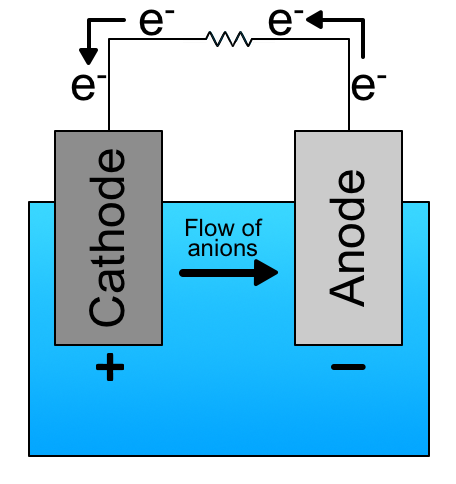
\includegraphics[width=0.5\textwidth]{ch2-pastwork/images/echemschem.png}
    \caption[Schematic of an electrochemical cell during discharge.]{Schematic of an electrochemical cell during discharge, with electrodes and flow of electrons and anions labeled.}
    \label{fig:echemschem}
\end{figure}


In battery literature, an oft-mentioned metric is the state of charge (SOC) which provides a measure of how much of the initial capacity of a battery still remains after a given amount of discharge. Typically, state of charge can be expressed as a percentage. A second, more complicated metric is the state of health (SOH). SOH (also expressed as a percentage) can be thought of as a measure of capacity fade, comparing the available total capacity for a given charge/discharge cycle to the initial total capacity. In this way, it functions like a time-resolved SOC. All batteries experience some capacity fade with use, and SOH is still a very difficult metric to measure directly. The last metric that is referenced often is the "C rate," written in the form C/2 or 2C. The "C" in this metric refers to the cell capacity in ampere-hours (Ah) or milli-ampere-hours (mAh), and the numeral refers to the inverse of the number of hours over which the capacity should be discharged. For example, C/2 would refer to a rate at which full capacity is discharged in two hours, while 2C refers to a rate at which cell capacity is discharged in 0.5 hours. Figure~\ref{fig:dischcurve} shows the difference between an ideal discharge curve, showing a constant voltage over the entire capacity of the cell, and an actual discharge curve, showing the non-idealities that come from ohmic, kinetic and mass transport limitations. Generally, the greater the discharge rate, the greater the slope of the discharge curve. A flatter discharge curve means that the voltage supplied is more constant, but this can make certain methods of state of charge estimation difficult. 

\begin{figure}[htb]
  \centering
    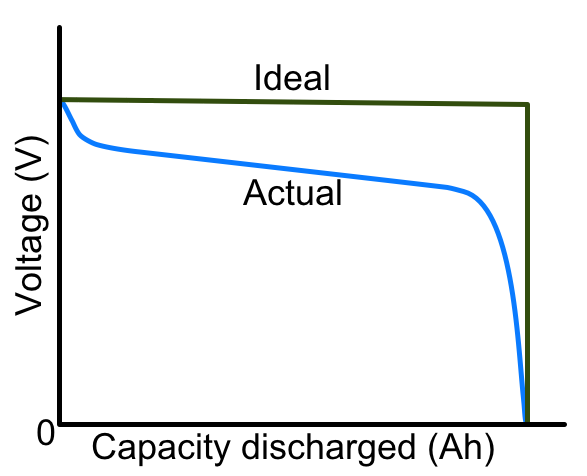
\includegraphics[width=0.5\textwidth]{ch2-pastwork/images/dischcurves.png}
    \caption[Example discharge curves.]{Example of an ideal and an actual discharge curve of a battery.}
    \label{fig:dischcurve}
\end{figure}

Many chemistries of both primary and secondary batteries exist. A common figure used to compare energy density and power density is the Ragone plot, shown for both primary and secondary batteries in Fig.~\ref{fig:ragone}.~\cite{ragone_primary,ragone_secondary} Ragone plots offer a straightforward method of narrowing down a battery chemistry based on energy or power needs. Furthermore, a cell's open circuit voltage can be estimated from a list of standard reduction potentials, which can further help to match a chemistry to an application.

\begin{figure}[htb]
  \centering
    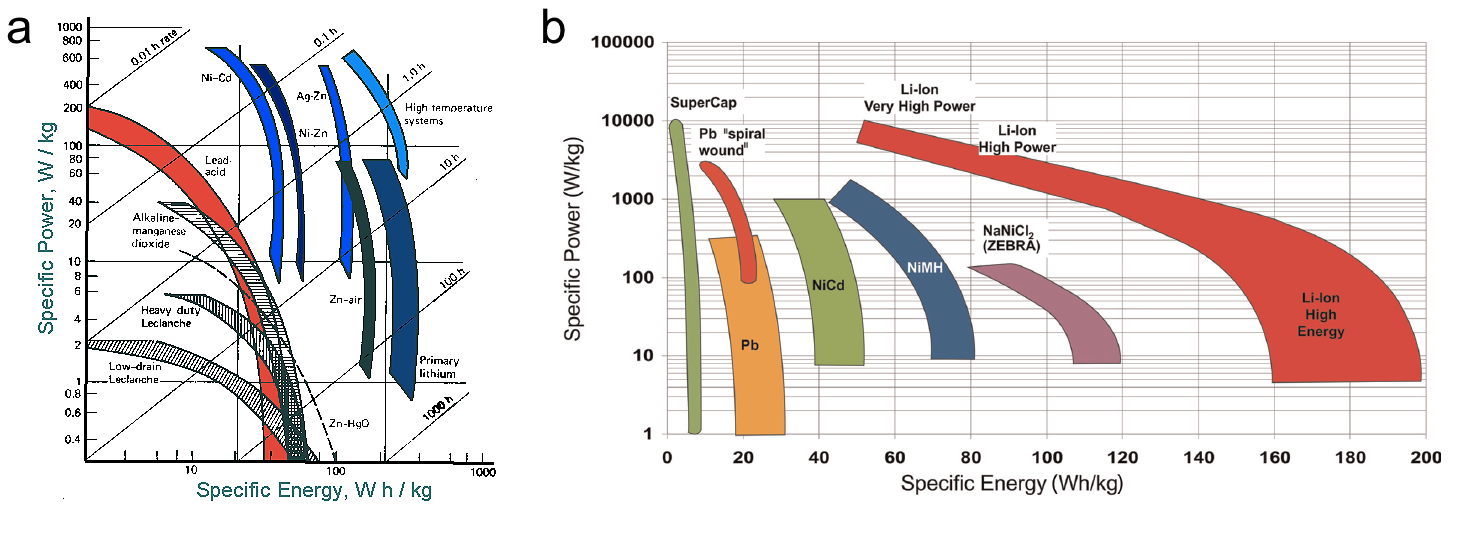
\includegraphics[width=\textwidth]{ch2-pastwork/images/ragone.png}
    \caption[Ragone plot of primary and secondary batteries.]{Ragone plot for \textbf{(a)} primary batteries, and \textbf{(b)} secondary batteries.}
    \label{fig:ragone}
\end{figure}

\subsection{Alkaline batteries}

The mainstay of the primary battery market is the alkaline battery, named for its use of KOH as an electrolyte. The chemistry and form factor have been popular for over 50 years because of the low cost of the source material (Zn) and the  bobbin cell design.~\cite{karl_patent} The bobbin cell construction is demonstrated in Fig.~\ref{fig:aaschem} along with the typical method of cell assembly is detailed in Fig.~\ref{fig:cellassembly}.~\cite{fujitsu} 

\begin{figure}[htb]
  \centering
    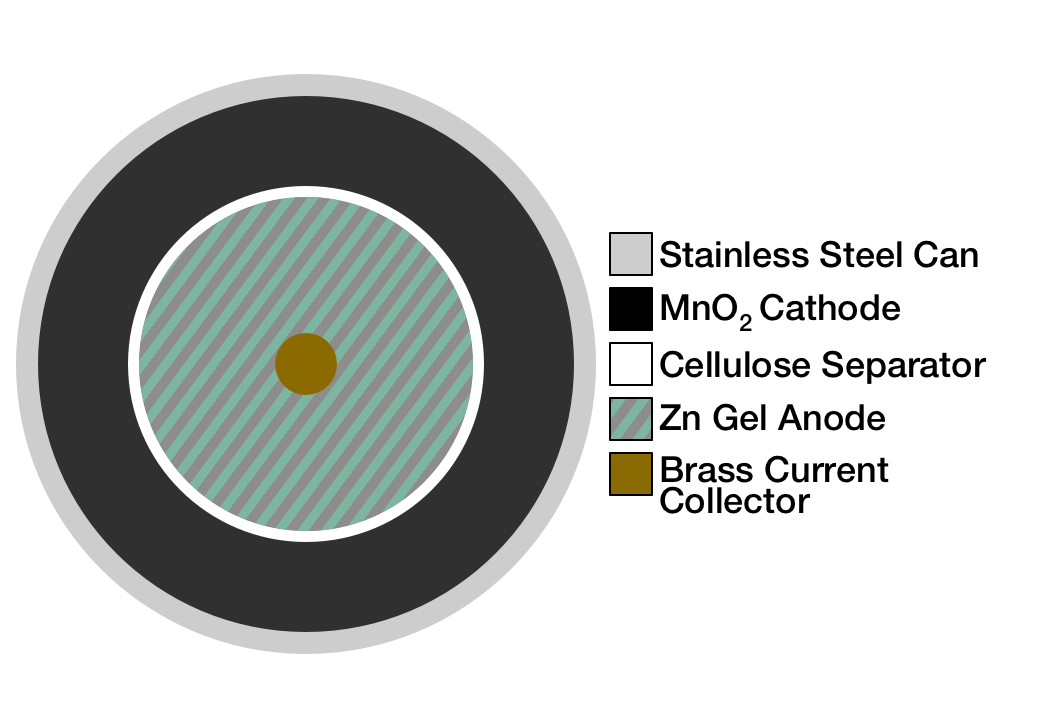
\includegraphics[width=0.60\textwidth]{ch3-dbb/Images/aaschem.png}
    \caption[Schematic of construction of an alkaline AA battery.]{Schematic of construction of an alkaline AA battery. Components are labeled according to the legend.}
    \label{fig:aaschem}
\end{figure}

\begin{figure}[htb]
  \centering
    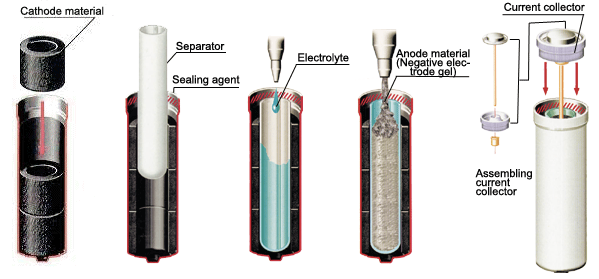
\includegraphics[width=\textwidth]{ch2-pastwork/images/cellassembly.png}
    \caption[Assembly process of alkaline AA batteries.]{Assembly process of alkaline AA batteries.}
    \label{fig:cellassembly}
\end{figure}

Each cell comprises a stainless steel can containing concentric layers of a \ce{MnO_2} cathode, a cellulose separator, a Zn gel anode containing KOH and a gelling agent, and a central brass current collecting pin. It is available in a number of sizes, with the most common sizes being the AA, AAA, C and D cell specifications, with a nominal voltage of 1.5 V.~\cite{linden} As the cell is discharged, the Zn anode is oxidized to ZnO, while the \ce{MnO_2} cathode is reduced through proton insertion into a variety of discharge products ranging from \ce{MnOOH} to \ce{ZnMn2O4}, depending on discharge rate.~\cite{Gallaway2015-xy}


\subsection{Lithium-ion batteries}

If alkaline batteries are the mainstays of the primary battery market, then lithium-ion batteries (LIBs) are almost certainly the equivalent mainstay of the secondary battery market. Popularized by consumer electronics and electric vehicles, LIBs offer some of the highest energy densities of current electrochemical storage methods.~\cite{linden}. A wide range of chemistries exist, and most LIBs have a wound construction in which layers of anode, polymeric separator, cathode, and current collector films are assembled in a stack and then wound to produce a final geometry, as demonstrated in Fig.~\ref{fig:libgeom}. Cells can be wound in a prismatic fashion to produce ``pouch" cells that have a rectangular cross section, or in a cylindrical fashion to produce ``jelly roll" cells. The former is most commonly used in portable electronic devices, while the latter has found use in laptop computers and electric vehicles such as the Tesla Model S.

\begin{figure}[htb]
  \centering
    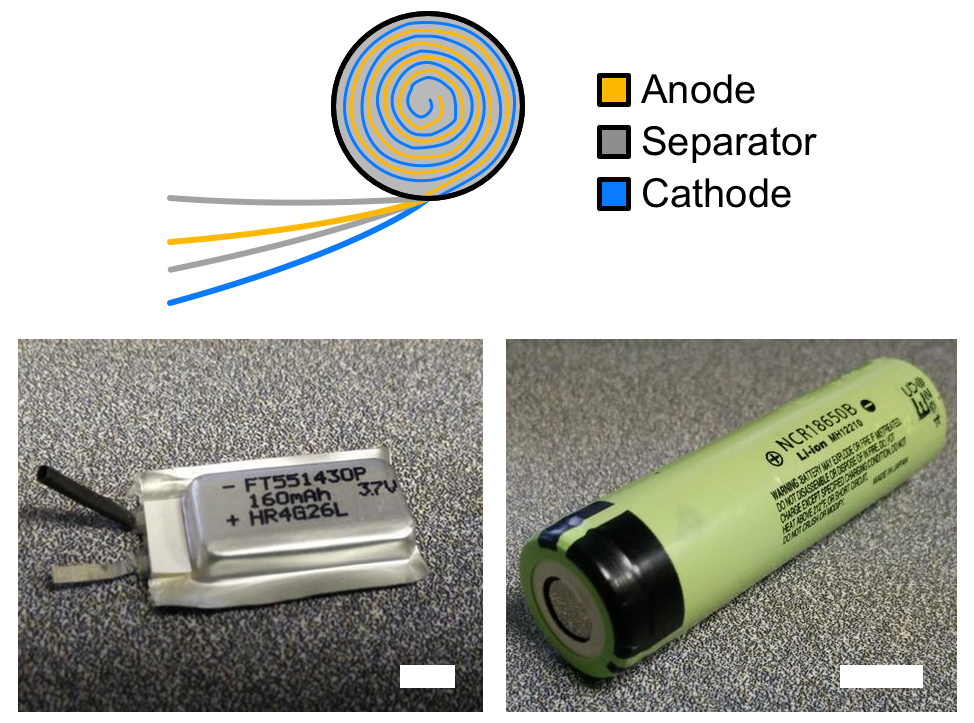
\includegraphics[width=0.8\textwidth]{ch2-pastwork/images/libgeom.png}
    \caption[Lithium-ion battery geometries.]{\textbf{(Top)} Schematic of a wound lithium-ion battery. \textbf{(Left)} \ce{LiCoO2} pouch cell.\textbf{(Right)} \ce{Li(NiCoAl)O2} ``jelly roll" cell.}
    \label{fig:libgeom}
\end{figure}

LIBs typically operate between 2.5 V and 4.2 V, with an average voltage of 3.7 V.~\cite{linden} Charging and discharging occur via a reversible intercalation process: during charge, lithium ions intercalate within the layers of the anode material, while during discharge, lithium ions intercalate into the cathode material while donating electrons to an external load. The typical anode material used in LIBs is graphite, owing to its layered structure. A considerable number of cathode chemistries exist, but this dissertation discusses only two of them: \ce{LiCoO2} and \ce{Li(NiCoAl)O2}. Both are layered oxides, but \ce{LiCoO2} has a slightly higher voltage vs. Li (3.9 V) while \ce{Li(NiCoAl)O2} has a higher specific capacity (200 mAh/g).~\cite{linden} 



\section{Electrical characterization techniques}
\label{sec:pastwork:echaracterization}
\section{Mechanical characterization techniques}
\label{sec:pastwork:mcharacterization}



\chapter{Dynamic mechanical testing of alkaline AA batteries relating coefficient of restitution and state of charge\label{ch:dbb}}

\section{Introduction}
\label{sec:alkbw:intro}

As discussed in Chapter~\ref{ch:dbb}, the LR6 Zn-MnO2 alkaline AA battery has been the mainstay of the primary battery market for nearly 60 years.~\cite{karl_patent} The low cost and abundance of the source materials have made alkaline AA batteries one of the most ubiquitous electrochemical energy storage cells, with over 40 million kgs sold in 2013 alone.~\cite{highbeam,ibisworld} Despite this ubiquity, there is still much to be learned about the materials properties of this system. Numerous studies have been performed \textit{ex situ} on Zn and \ce{MnO2} in alkaline solutions to understand the processes that occur at each electrode.\cite{arise,Balachandran2002-vd,Chen1993-bw,Chin1982-lw,Kozawa1966-ga,Kozawa1965-yt,Liu1981-ub,McLarnon1991-bw,Pandya1995-tg} In addition, \textit{ex situ} mechanical testing has shown that microscopic morphological changes in the Zn anode can affect a macroscopic change in the mechanical response of the full cell, as detailed in Chapter~\ref{ch:dbb}.~\cite{Bhadra2015-aq} Thus far, however, \textit{in operando} efforts have been limited to either neutron tomography,~\cite{Manke2007-yj,Riley2010-ur} or large scale experiments using synchrotron sources to perform EDXRD,~\cite{gallaway,Gallaway2015-xy} or x-ray microtomography.~\cite{haibel, Manke2007-yj}

In Chapter~\ref{ch:bw}, we demonstrated a technique which was applicable to most battery chemistries and provided in operando monitoring of both state of charge and state of health through non-destructive mechanical interrogation: EAToF.~\cite{Hsieh2015-kr} This method uses an ultrasonic contact transducer to generate an acoustic pulse. The resulting pulse will display different ToF profiles based on the sound speed of the battery component materials. Sound speed, \emph{c}, in a material scales with the bulk modulus, \emph{B}, and inversely with the density, \emph{$\rho$} as shown previously in Equation~\ref{eq:newtonlaplace}, and as both of these materials properties change as a function of state of charge and state of health we can use the ToF profiles to analyze the state of the battery.

\begin{equation*}
c= \sqrt{\frac{B}{\rho}}
\tag{\ref{eq:newtonlaplace}}
\end{equation*}

In this chapter, we applied EAToF measurements to LR6 alkaline AA batteries. The LR6 uses a unique bobbin geometry, detailed previously in Fig.~\ref{fig:aaschem}, in which each electrode occupies a large contiguous volume within the cell, unlike in jelly roll geometries where thin electrode layers are rolled to fill the cylindrical or prismatic volume. As a result, there are relatively few interfaces for scattering of the ultrasonic pulse and ample regions of each material through which the pulse can travel. In alkaline AA batteries, the relevant density and modulus shifts are strongest in the Zn anode due to a densification and dehydration of the initial Zn gel into a porous ZnO solid which occurs radially beginning at the separator and progressing inwards to the central current collecting pin.~\cite{Bhadra2015-aq} This transition results in a 39\% change in density and a 107\% change in bulk modulus based on the materials property information in Table 1. EAToF allows us to see this densification of the anode due to oxidation during discharge but also offers more insight into the quality of the anode materials, which we demonstrate by performing EAToF measurements on a number of brands of alkaline AA batteries. We show that cells displaying greater discharge capacity also have pronounced differences in the EAToF transmission profiles of their respective anodes.

\begin{figure}[htb]
  \centering
    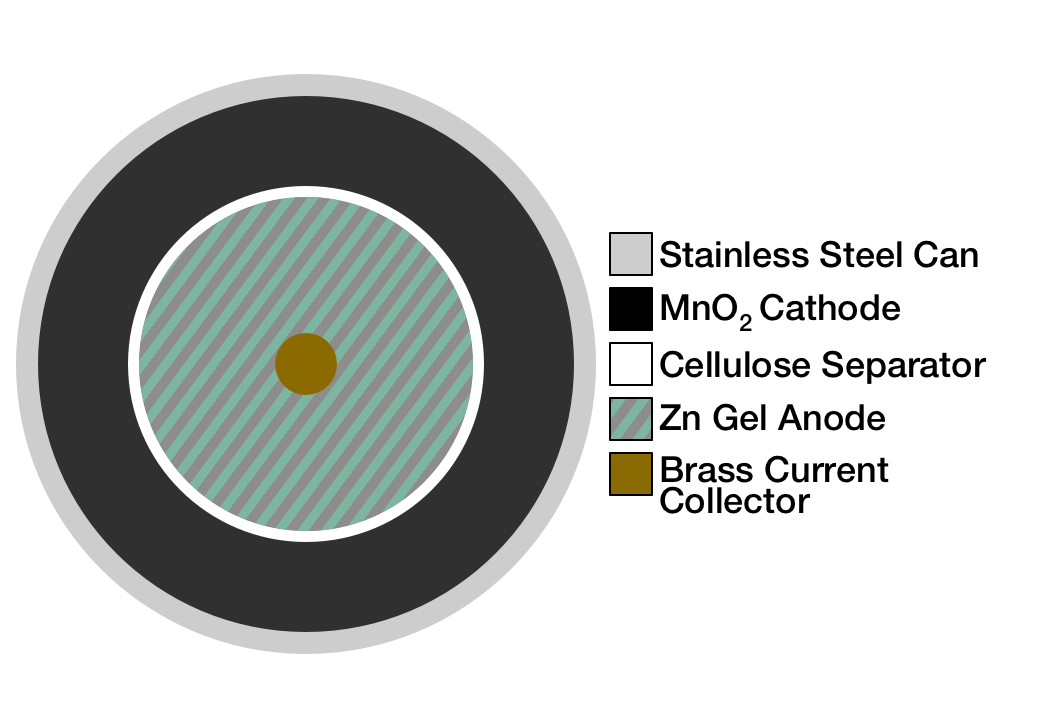
\includegraphics[width=0.80\textwidth]{ch3-dbb/Images/aaschem.png}
    \repeatcaption{fig:aaschem}{Schematic of construction of a alkaline AA battery. Components are labeled according to the legend.}
\end{figure}

\begin{table}[htb]
\centering
  \repeatcaptiont{tab:table3}{Materials properties of electrode materials in an alkaline battery}
  \begin{tabular}{*{4}{l}}
    \hline
    Material & Density (g/cm$^3$) & Bulk modulus (GPa) & Reference\\
    \hline
        Zinc (Zn)& 7.05 & 72.0 & ~\cite{Kaye2014-am}\\
        Zinc oxide (ZnO) & 5.06 & 134.0 & ~\cite{Munro2002-pg}\\
        Zn gel & 3.64 (est.) & 57.6 (est.) & ~\cite{Kaye2014-am,Murei2007-ke}\\
        Electrolytic (\ce{MnO2}) & 4.55 & 54.5 & ~\cite{Robert1990-zl,Tao2013-vg}\\
        Groutite (MnOOH) & 4.14 & 39.8 & ~\cite{Robert1990-zl,Tao2013-vg}\\
  \end{tabular}
\end{table}



\section{Experimental methods}
\label{sec:bw:exp}
\label{sec:dbb:results}

\section{Morphology characterization and coefficient of restitution evolution during discharge}
As an alkaline battery is discharged, the anode undergoes oxidation from Zn to ZnO, as seen in Eq.~\ref{eq:zn1} and~\ref{eq:zn2}, while the cathode is reduced from {\ce{MnO_2}} to MnOOH, shown in Eq.~\ref{eq:mn}.

\begin{equation}
{\ce{Zn + 4OH^- -> Zn(OH)^{2-}_{4} + 2e^-}}
\label{eq:zn1}
\end{equation}
\begin{equation}
{\ce{Zn(OH)^{2-}_{4} -> ZnO + H_{2}O + 2OH^-}}
\label{eq:zn2}
\end{equation}
\begin{equation}
{\ce{MnO_{2} + H_{2}O + e- -> MnOOH + OH^-}}
\label{eq:mn}
\end{equation}

\noindent Equation~\ref{eq:zn1} shows that the battery produces {\ce{Zn(OH)^{2-}_{4}} ions in solution until the electrolyte becomes supersaturated, at which point it begins to precipitate as ZnO ~\cite{linden}.

\textit{Post mortem} analysis shows that in alkaline AA batteries, the Zn gel anode initially exists as discrete Zn particles in a matrix of KOH electrolyte and a gelling agent. After discharge, the anode densifies into a porous ZnO solid that appears more compact closer to the separator, as shown in Fig.~\ref{fig:SEM}. The densification of the anode affects the mechanical properties of the battery. The COR, which measures the elasticity of a collision between two objects, is one such mechanical property that can be determined as shown in Eq.~\ref{eq:cor}.



\begin{figure}[htb]
  \centering
    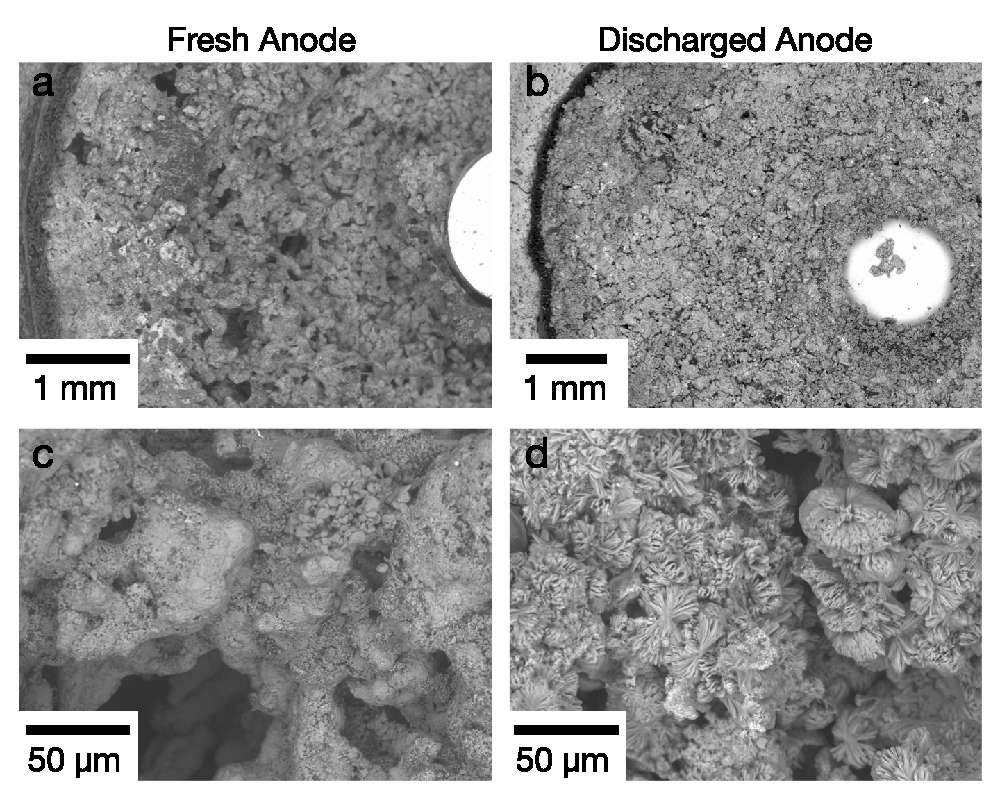
\includegraphics[width=0.8\textwidth]{ch3-dbb/Images/ZnSEM.eps}
    \caption[SEM images of sectioned fresh and fully discharged alkaline batteries]{a) SEM image of ``fresh" cell. b) SEM image of the same cell after full discharge (2850 mAh passed). c) High mag. SEM image showing fresh Zn particles. d) High mag. SEM image showing coagulated ZnO particles after full discharge.}
    \label{fig:SEM}
\end{figure}

\begin{equation}
COR = \frac{1}{N} \sum\limits_{n=1}^N \sqrt{\frac{h_{n+1}}{h_n}}
\label{eq:cor}
\end{equation}

\noindent where \(N\) is the number of bounces, and \(h\) denotes the bounce heights determined from Eq.~\ref{eq:bounce}. Using the bounce test described previously, the COR of alkaline batteries was measured through full discharge.

Figure~\ref{fig:COR1to3} shows the evolution of the COR for three identical AA cells as capacity is passed in increments of 280 milliamp-hours (mAh) at 280 mA, corresponding to a rate of C/10. The inset shows a composited image of the corresponding drop tests for a single cell. A sharp increase in COR occurs at 80\% SOC, when 560 mAh have passed, followed by asymptotic leveling of the COR at a value of 0.66\(\pm\) 0.02 after 50\% SOC (1400 mAh passed).  The three cells show excellent agreement in the low and high COR regimes, and the variance in the dynamic regime (80\% to 50\% SOC) shows that there is some variance from cell to cell in ZnO growth.

\clearpage

\begin{figure}[hbt]
  \centering
    \includegraphics[width=0.8\textwidth]{ch3-dbb/Images/cor280.pdf}
    \caption[Coefficient of restitution evolution at 280 mA.]{Coefficient of restitution as a function of capacity passed at 280 mA. Inset: Composited image of bounce behavior for a single cell over full depth of discharge}
    \label{fig:COR1to3}
\end{figure}

To show the transition between the low COR and high COR regimes more clearly and to gauge the effect of discharge rate on the COR evolution, cells were discharged at 50 mA in one hour intervals (50 mAh) prior to bounce testing, corresponding to a rate of roughly C/57. As shown in Figure~\ref{fig:50mah} the COR is constant for low depths of discharge, similar to the cells discharged at 280 mA. The rise in COR begins after 450 mAh have been passed, which is roughly 100 mAh earlier than in the cells discharged at 280 mA. The leveling of COR for these cells occurs at 950 mAh passed, which is roughly 450 mAh earlier than the saturation point for COR of cells discharged at 280 mA. It has been shown previously by Horn et al~\cite{horn} that lower discharge rates will result in a more even distribution of ZnO in the anode, compared to that of a higher discharge rate, thus a more even distribution of ZnO. We posit that because ZnO is the major contributor to the changes in mechanical properties of the battery, a more even distribution results in earlier leveling of the COR.

\begin{figure}[ht]
  \centering
    \includegraphics[width=0.8\textwidth]{ch3-dbb/Images/50mAh.eps}
    \caption[Coefficient of restitution evolution at 50 mA.]{Coefficient of restitution as a function of capacity passed at 50 mA in 50 mAh increments.}
    \label{fig:50mah}
\end{figure}


\section{Possible reasons for COR evolution}

As the stainless steel casing does not change or partake in the electrochemical reaction, four possible effects associated with discharging an alkaline battery may be correlated with the observed change in COR: 1) mass loss, 2) reduction of the cathode from {\ce{MnO_2}} to {\ce{MnOOH}}, 3) water consumption, and 4) oxidation of the anode from Zn to ZnO. We will discuss each of these possibilities in the remainder of the chapter. 

\subsection{Mass loss and cathode reduction}

Mass loss can be discounted, as under all operating conditions no change was observed in the mass of each battery. The cells are effectively sealed, but have safety valves to handle \ce{H2} generation which results from corrosion of the zinc,~\cite{linden} and again, no mass loss was measured during the experiments. 

The EDXRD spectra for the {\ce{MnO_2}} cathode shows peak shifts that begin immediately upon discharge, at least 400 mAh before the onset of COR increase, as shown in Figure~\ref{fig:mno2}. As reduction of the cathode is a linear process, it does not correlate clearly with the non-linear increase in COR.

\begin{figure}[htb]
\centering
    \includegraphics[width=0.8\textwidth]{ch3-dbb/Images/MnO2XRD.eps}
    \caption[Representative \ce{MnO2} EDXRD spectra at 100 mA discharge rate.]{Representative \ce{MnO2} EDXRD spectra at 100 mA discharge rate.}
    \label{fig:mno2}
\end{figure}

\subsection{Water consumption and ZnO formation}

Analysis of the discharge reaction and physical properties of water, Zn, and ZnO reveals that these two aspects are strongly coupled.  While the density of ZnO (5.61 g/cm\(^3\)) is less than that of Zn (7.14 g/cm\(^3\)), the density of water with 8.9 M KOH is 1.41 g/cm\(^3.\)  Complicating the system is the use of proprietary blends of gelation agents added to the anode (typically combinations of cellulose and polyethylene glycol), so we will assume a composite density of 1.40 g/cm\(^3.\)~\cite{linden}  Equations~\ref{eq:zn1},~\ref{eq:zn2}, and~\ref{eq:mn} show that for every mole of Zn eventually oxidized to ZnO, and every mole of {\ce{MnO_2}} reduced to MnOOH, one mole of \ce{H2O} must be consumed.  This means that for 2800 mAh of charge passed, 0.94 g of \ce{H2O} must be consumed between the protonation of the {\ce{MnO_2}} and the oxidation of the zinc. 

We devised the following test to determine if water removal, without ZnO conversion, caused the increase in COR:  three AA cells, one at 100\% SOC (as-received), 50\% SOC (half-discharged), and 0\% SOC (fully-discharged), were modified by removing the top 1 cm$^2$ of casing, exposing both the anode and cathode.  The COR of cell was then measured once before and again after dehydration in a vacuum oven at 25\celsius~for 72 hours.

To ensure that water was removed from the entire cell (and not just the cathode), we then ran a separate test where 1 g of zinc anode gel was removed before and after desiccation. Each sample (as received and desiccated at each state of charge) was held at 80\celsius~for 24 hours. The zinc gel, before our desiccation method, lost 0.2 $\pm$ 0.002 g when dried at 80\celsius~in vacuum. The zinc gels, after desiccation, lost negligible (lower than the scale precision) amounts of water.  This gave us confidence that water was removed through the cell during our 25\celsius~desiccation. Additionally, the non-desiccated zinc gel could be "spread" readily with a spatula; in contrast, the desiccated zinc was rigid and would crumble when enough shear was applied to move the particles. Both were notably different from the discharged zinc, which was a rigid, concrete-like mass that was difficult to break apart. 

Removing the case decreased the overall coefficient of restitution. Table~\ref{tab:cortable} indicates that there was no meaningful change in the COR when the cells at different states of charge were dehydrated at 25\celsius~for three days, despite the aforementioned water loss and "stiffening" of the anode. Thus, water removal from the cell, and particularly from the zinc gel anode, alone does not alter the COR of the cell.


\begin{table}[htb]
\centering
 \caption{\label{tab:cortable}Water content effect on coefficient of restitution.}
  \begin{tabular}{p{2.5cm}p{2.5cm}p{2.5cm}p{2.5cm}}
    \hline
    & Coefficient of restitution at 100\% SOC & Coefficient of restitution at 50\% SOC & Coefficient of restitution at 0\% SOC\\
    \hline
        As received & 0.10 $\pm$ 0.05 & 0.43 $\pm$ 0.02 & 0.43 $\pm$ 0.02\\
        Dehydrated & 0.10 $\pm$ 0.05 & 0.43 $\pm$ 0.02 & 0.42 $\pm$ 0.02\\
        Unmodified & 0.23 $\pm$ 0.02 & 0.60 $\pm$ 0.03 & 0.66 $\pm$ 0.02\\
  \end{tabular}
\end{table}

What is more likely the cause of the increased COR is is a combination of water being consumed as zinc oxide forms as indicated by reactions 1 and 2.  What we will show in subsequent sections is that while water is consumed to form zinc oxide throughout the anode, the COR change appears to correlate with the point at which ZnO is present through the thickness of the the Zn gel anode.

\section{Comparison of bounce test data to \textit{in situ} data}

\subsection{Comparison to electrochemical impedance spectroscopy data}

One method for measuring the evolution of interfaces within a battery is electrochemical impedance spectroscopy (EIS).~\cite{dornbusch,ghavami} EIS was performed after every 10\% of capacity discharged (280 mAh) to observe the effects of anode oxidation on the impedance of the battery. We found a high value for the imaginary (Z") and  real (Z') components of impedance in the as-received battery, with a two order of magnitude drop in both following 10\% discharge of the cell. This drop was most evident in the low frequency regime of the EIS spectra, often associated with mass transport limitations. We believe this high initial impedance of the cell is related to a proprietary polymeric coating on the zinc anode used in this brand of battery to improve the shelf life.  It was confirmed that while other brands of alkaline AA batteries do not have this high initial electrochemical impedance, they do exhibit the same increase in COR as a function of depth of discharge. These results, while of interest, do not give a clear indication of the cause of the increase and leveling of the COR. While not crucial to our hypothesis, a detailed discussion of the EIS model that was developed is presented along with references to established EIS models in Appendix~\ref{ch:eis}. EIS suggests that some structural evolution occurs within the anode, but a method is required to characterize discrete volumes within the battery to understand the oxidation process.  

\subsection{Comparison to EDXRD data}

Recent studies have shown that performing \textit{in situ} EDXRD on batteries during discharge can probe the evolution of the internal components.~\cite{gallaway,haibel,Manke2007-yj} Using similar methods, \textit{in situ} EDXRD was performed in AA batteries at three discharge rates: 100 mA, 200 mA, and 300 mA. The x-ray beam was incident along the width of the battery, which allows for collection of spatially resolved data, providing a measure of the oxidation of Zn to ZnO at both edges of the anode: the separator and the current collector. In all three cells, we see that ZnO forms at the separator interface (Fig.~\ref{fig:znxrd}a,c,e) before forming at the current collector interface (Fig.~\ref{fig:znxrd}b,d,f). The capacity passed at which ZnO is present at each interface is detailed in Table~\ref{tab:znotable}.

\begin{table}[htb]
\centering
  \caption{\label{tab:znotable}Formation of ZnO within the anode.}
  \begin{tabular}{*{3}{l}}
    \hline
       Discharge rate (mA)&\specialcell{Capacity passed before\\appearance of ZnO\\at separator (mAh)}&\specialcell{Capacity passed before\\appearance of ZnO\\at current collector (mAh)}\\
    \hline
        100 & 200 - 300 & 300 - 400\\
        200 & 200 - 400 & 400 - 600\\
        300 & 300 - 600 & 300 - 600\\
  \end{tabular}
\end{table}


These spectra confirm the results of Horn et al,~\cite{horn} who have shown that at higher discharge rates, ZnO will grow preferentially at the separator interface before growing through the anode towards the current collector. They have found that ZnO initially grows as a shell around the Zn particles (Type I ZnO) through solution-precipitation of {\ce{Zn(OH)^{2-}_{4}}. Once the particle is completely enveloped in Type I ZnO it begins to oxidize and deposit onto the the inside surface of the Type I ZnO shell via a second solution-precipitation step (Type II ZnO). Based on the EDXRD spectra in Fig.~\ref{fig:znxrd}, the oxidation of Zn in the cell ultimately forms a percolation network of ZnO from the separator to the current collector, and because of the axial symmetry of the cell, detection of radial percolation also suggest percolation throughout the entire cell. This agrees well with the results of Arise et al.,~\cite{arise} who have shown that following initial precipitation of ZnO onto the anode surface, the particles will coarsen and form dense films. It is also supported by the \textit{in situ} x-ray microtomography performed by Haibel et al.,~\cite{haibel}, who show that the growth front of ZnO in an alkaline cell travels from the separator to the current collecting pin as a function of depth of discharge.

\figskip{fig:znxrd}

\begin{figure}[htb]
\centering
    \includegraphics[width=\textwidth]{ch3-dbb/Images/FullZnXRD.eps}
    \caption[XRD progression of anode at separator and current collector interfaces at 100 mA, 200 mA, and 300 mA discharge rates.]{XRD progression of anode at separator and current collector interfaces at \textbf{(a,b)} 100 mA, \textbf{(c,d)} 200 mA, and \textbf{(e,f)} 300 mA discharge rates. ZnO peaks are denoted by green dashed lines, and Zn peaks are denoted by red dashed lines.}
    \label{fig:znxrd}
\end{figure}
\clearpage

Comparing the bounce test data presented in Fig.~\ref{fig:COR1to3} with the EDXRD spectra in Fig.~\ref{fig:znxrd}, it is clear that the formation of this percolation pathway occurs at the same time that the COR increases. This hypothesis is supported by the use of ZnO as an industrial additive to increase the COR of materials,~\cite{nesbitt_golf} and previous studies performed on ceramic/metal composites (cermets),~\cite{hussainova} in which increasing the ceramic content of a cermet will result in an increase in the COR, assuming the ceramic has a higher elastic modulus relative to the metal matrix. Table 3 shows relevant materials properties for the alkaline battery system. Treating the partially oxidized anode as a cermet, and knowing that the Zn to ZnO transition results in 107\% increase in bulk modulus, we expect an increase in COR as the Zn particles are oxidized.


\begin{table}[htb]
\centering
  \caption{\label{tab:table3}Materials properties of electrode materials in an alkaline battery}
  \begin{tabular}{*{4}{l}}
    \hline
    Material & Density (g/cm$^3$) & Bulk modulus (GPa) & Reference\\
    \hline
        Zinc (Zn)& 7.05 & 72.0 & ~\cite{Kaye2014-am}\\
        Zinc oxide (ZnO) & 5.06 & 134.0 & ~\cite{Munro2002-pg}\\
        Zn gel & 3.64 (est.) & 57.6 (est.) & ~\cite{Kaye2014-am,Murei2007-ke}\\
        Electrolytic (\ce{MnO2}) & 4.55 & 54.5 & ~\cite{Robert1990-zl,Tao2013-vg}\\
        Groutite (MnOOH) & 4.14 & 39.8 & ~\cite{Robert1990-zl,Tao2013-vg}\\
  \end{tabular}
\end{table}


% \begin{table}[h]
%     \centering
%         \caption{\label{tab:table3}Materials Properties}
%         \begin{tabular}{lll}
%             Material & Density (g/cm$^3$)~\cite\{EncOfMat\} & Bulk Modulus (GPa)\\
%             Zinc (Zn) & 7.05 & 59~\cite\{Ledbetter1977-rl\} \\
%             Zinc oxide (ZnO) & 5.06 & 134~\cite\{Munro2002-pg\}    \\
%             Ramsdellite (\ce\{MnO2\}) & 4.37\ & 119~\cite\{Lin2011-ur\}   \\
%             Groutite (MnOOH)          & 4.14\ & 96~\cite\{Suzuki2013-dt\}   
%         \end{tabular}
% \end{table}

The leveling of the COR is best explained using the methods of Antonyuk et al.,~\cite{antonyuk} who have found that a material's COR will saturate at the point at which it no longer yields plastically. Using Faradaic analysis, after 1400 mAh of charge is passed (50\% SOC), 1.71 g of Zn will be consumed at the anode, while 2.13 g of ZnO will be produced. At this state of charge half the Zn has been converted to ZnO, assuming a zinc limited battery, making ZnO the majority phase in the anode, both volumetrically and gravimetrically. As per Horn et al and Arise et al.,~\cite{horn,arise} the Type I ZnO shells will form together and sequester the liquid electrolyte while there is remaining free volume within the anode, while the bulk of the Zn particle will be oxidized to Type II ZnO. Initially, the anode gel consists of discrete Zn particles that can move within the gel matrix. Once percolation begins, this motion becomes suppressed. Once the anode densifies, as shown in Figure 1b, it becomes a stiff ceramic core that arrests all movement of the discrete Zn particles, and the COR levels off. This process is detailed in Fig.~\ref{fig:sketch}, which shows the initial gel, the growth of Type I ZnO, the percolation of ZnO in the anode, and the final densification of the anode.
\begin{figure}[h]
  \centering
    \includegraphics[width=0.8\textwidth]{ch3-dbb/Images/dbbsketch.eps}
    \caption[The progression of ZnO formation in the alkaline AA anode]{The progression of ZnO formation in the anode. \textbf{(a)} The initial anode gel comprised of Zn particles in an electrolyte/cellulose matrix. \textbf{(b)} Formation of Type I ZnO shells on Zn particles. c) Formation of a percolation pathway. \textbf{(d)} Densification of the anode.}
    \label{fig:sketch}
\end{figure}
\section{Conclusions}
\label{sec:alkbw:conclusion}





\chapter{A general method for ultrasonic interrogation of batteries\label{ch:bw}}

\section{Introduction}
\label{sec:alkbw:intro}

As discussed in Chapter~\ref{ch:dbb}, the LR6 Zn-MnO2 alkaline AA battery has been the mainstay of the primary battery market for nearly 60 years.~\cite{karl_patent} The low cost and abundance of the source materials have made alkaline AA batteries one of the most ubiquitous electrochemical energy storage cells, with over 40 million kgs sold in 2013 alone.~\cite{highbeam,ibisworld} Despite this ubiquity, there is still much to be learned about the materials properties of this system. Numerous studies have been performed \textit{ex situ} on Zn and \ce{MnO2} in alkaline solutions to understand the processes that occur at each electrode.\cite{arise,Balachandran2002-vd,Chen1993-bw,Chin1982-lw,Kozawa1966-ga,Kozawa1965-yt,Liu1981-ub,McLarnon1991-bw,Pandya1995-tg} In addition, \textit{ex situ} mechanical testing has shown that microscopic morphological changes in the Zn anode can affect a macroscopic change in the mechanical response of the full cell, as detailed in Chapter~\ref{ch:dbb}.~\cite{Bhadra2015-aq} Thus far, however, \textit{in operando} efforts have been limited to either neutron tomography,~\cite{Manke2007-yj,Riley2010-ur} or large scale experiments using synchrotron sources to perform EDXRD,~\cite{gallaway,Gallaway2015-xy} or x-ray microtomography.~\cite{haibel, Manke2007-yj}

In Chapter~\ref{ch:bw}, we demonstrated a technique which was applicable to most battery chemistries and provided in operando monitoring of both state of charge and state of health through non-destructive mechanical interrogation: EAToF.~\cite{Hsieh2015-kr} This method uses an ultrasonic contact transducer to generate an acoustic pulse. The resulting pulse will display different ToF profiles based on the sound speed of the battery component materials. Sound speed, \emph{c}, in a material scales with the bulk modulus, \emph{B}, and inversely with the density, \emph{$\rho$} as shown previously in Equation~\ref{eq:newtonlaplace}, and as both of these materials properties change as a function of state of charge and state of health we can use the ToF profiles to analyze the state of the battery.

\begin{equation*}
c= \sqrt{\frac{B}{\rho}}
\tag{\ref{eq:newtonlaplace}}
\end{equation*}

In this chapter, we applied EAToF measurements to LR6 alkaline AA batteries. The LR6 uses a unique bobbin geometry, detailed previously in Fig.~\ref{fig:aaschem}, in which each electrode occupies a large contiguous volume within the cell, unlike in jelly roll geometries where thin electrode layers are rolled to fill the cylindrical or prismatic volume. As a result, there are relatively few interfaces for scattering of the ultrasonic pulse and ample regions of each material through which the pulse can travel. In alkaline AA batteries, the relevant density and modulus shifts are strongest in the Zn anode due to a densification and dehydration of the initial Zn gel into a porous ZnO solid which occurs radially beginning at the separator and progressing inwards to the central current collecting pin.~\cite{Bhadra2015-aq} This transition results in a 39\% change in density and a 107\% change in bulk modulus based on the materials property information in Table 1. EAToF allows us to see this densification of the anode due to oxidation during discharge but also offers more insight into the quality of the anode materials, which we demonstrate by performing EAToF measurements on a number of brands of alkaline AA batteries. We show that cells displaying greater discharge capacity also have pronounced differences in the EAToF transmission profiles of their respective anodes.

\begin{figure}[htb]
  \centering
    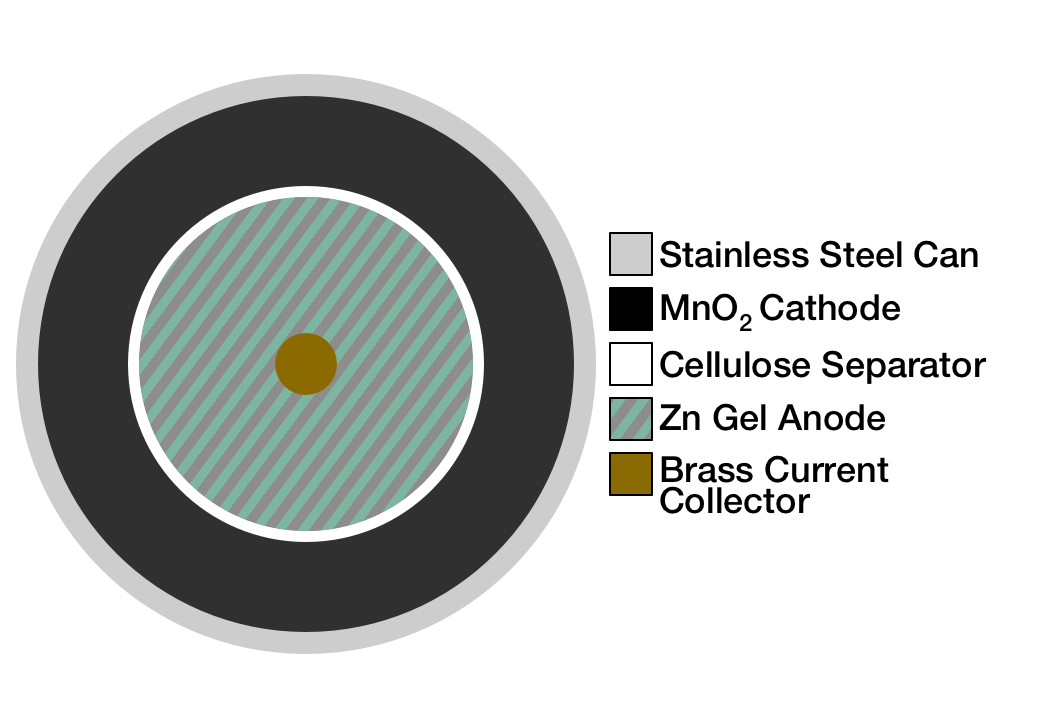
\includegraphics[width=0.80\textwidth]{ch3-dbb/Images/aaschem.png}
    \repeatcaption{fig:aaschem}{Schematic of construction of a alkaline AA battery. Components are labeled according to the legend.}
\end{figure}

\begin{table}[htb]
\centering
  \repeatcaptiont{tab:table3}{Materials properties of electrode materials in an alkaline battery}
  \begin{tabular}{*{4}{l}}
    \hline
    Material & Density (g/cm$^3$) & Bulk modulus (GPa) & Reference\\
    \hline
        Zinc (Zn)& 7.05 & 72.0 & ~\cite{Kaye2014-am}\\
        Zinc oxide (ZnO) & 5.06 & 134.0 & ~\cite{Munro2002-pg}\\
        Zn gel & 3.64 (est.) & 57.6 (est.) & ~\cite{Kaye2014-am,Murei2007-ke}\\
        Electrolytic (\ce{MnO2}) & 4.55 & 54.5 & ~\cite{Robert1990-zl,Tao2013-vg}\\
        Groutite (MnOOH) & 4.14 & 39.8 & ~\cite{Robert1990-zl,Tao2013-vg}\\
  \end{tabular}
\end{table}



\section{Experimental methods}
\label{sec:bw:exp}
\label{sec:dbb:results}

\section{Morphology characterization and coefficient of restitution evolution during discharge}
As an alkaline battery is discharged, the anode undergoes oxidation from Zn to ZnO, as seen in Eq.~\ref{eq:zn1} and~\ref{eq:zn2}, while the cathode is reduced from {\ce{MnO_2}} to MnOOH, shown in Eq.~\ref{eq:mn}.

\begin{equation}
{\ce{Zn + 4OH^- -> Zn(OH)^{2-}_{4} + 2e^-}}
\label{eq:zn1}
\end{equation}
\begin{equation}
{\ce{Zn(OH)^{2-}_{4} -> ZnO + H_{2}O + 2OH^-}}
\label{eq:zn2}
\end{equation}
\begin{equation}
{\ce{MnO_{2} + H_{2}O + e- -> MnOOH + OH^-}}
\label{eq:mn}
\end{equation}

\noindent Equation~\ref{eq:zn1} shows that the battery produces {\ce{Zn(OH)^{2-}_{4}} ions in solution until the electrolyte becomes supersaturated, at which point it begins to precipitate as ZnO ~\cite{linden}.

\textit{Post mortem} analysis shows that in alkaline AA batteries, the Zn gel anode initially exists as discrete Zn particles in a matrix of KOH electrolyte and a gelling agent. After discharge, the anode densifies into a porous ZnO solid that appears more compact closer to the separator, as shown in Fig.~\ref{fig:SEM}. The densification of the anode affects the mechanical properties of the battery. The COR, which measures the elasticity of a collision between two objects, is one such mechanical property that can be determined as shown in Eq.~\ref{eq:cor}.



\begin{figure}[htb]
  \centering
    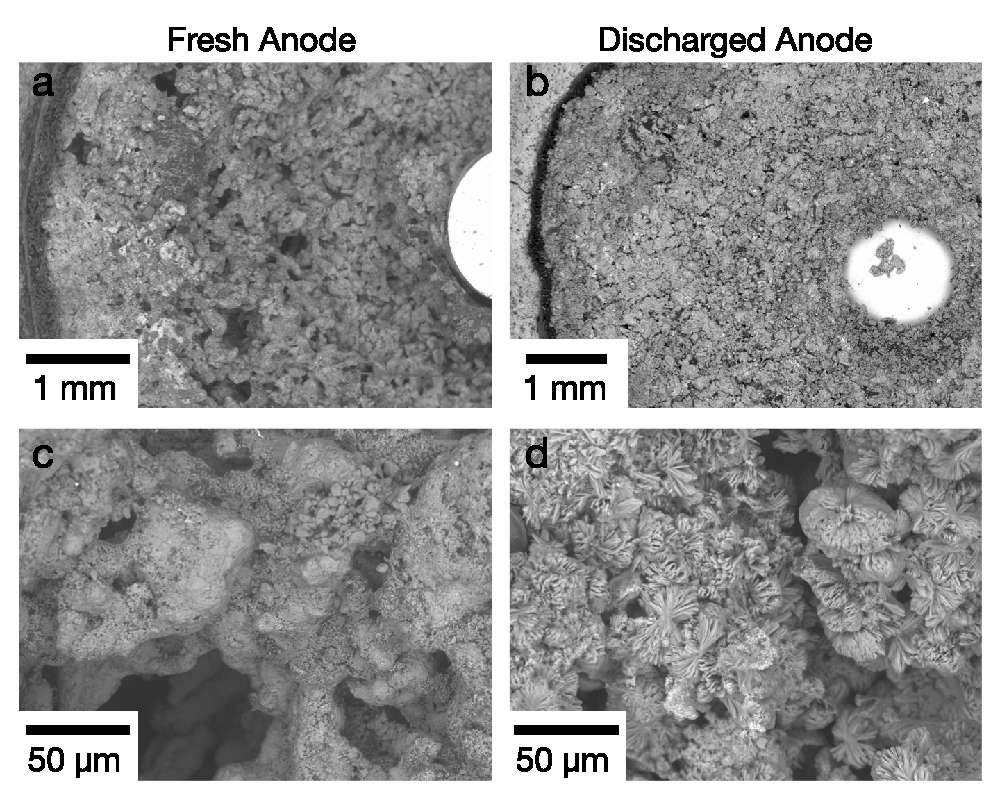
\includegraphics[width=0.8\textwidth]{ch3-dbb/Images/ZnSEM.eps}
    \caption[SEM images of sectioned fresh and fully discharged alkaline batteries]{a) SEM image of ``fresh" cell. b) SEM image of the same cell after full discharge (2850 mAh passed). c) High mag. SEM image showing fresh Zn particles. d) High mag. SEM image showing coagulated ZnO particles after full discharge.}
    \label{fig:SEM}
\end{figure}

\begin{equation}
COR = \frac{1}{N} \sum\limits_{n=1}^N \sqrt{\frac{h_{n+1}}{h_n}}
\label{eq:cor}
\end{equation}

\noindent where \(N\) is the number of bounces, and \(h\) denotes the bounce heights determined from Eq.~\ref{eq:bounce}. Using the bounce test described previously, the COR of alkaline batteries was measured through full discharge.

Figure~\ref{fig:COR1to3} shows the evolution of the COR for three identical AA cells as capacity is passed in increments of 280 milliamp-hours (mAh) at 280 mA, corresponding to a rate of C/10. The inset shows a composited image of the corresponding drop tests for a single cell. A sharp increase in COR occurs at 80\% SOC, when 560 mAh have passed, followed by asymptotic leveling of the COR at a value of 0.66\(\pm\) 0.02 after 50\% SOC (1400 mAh passed).  The three cells show excellent agreement in the low and high COR regimes, and the variance in the dynamic regime (80\% to 50\% SOC) shows that there is some variance from cell to cell in ZnO growth.

\clearpage

\begin{figure}[hbt]
  \centering
    \includegraphics[width=0.8\textwidth]{ch3-dbb/Images/cor280.pdf}
    \caption[Coefficient of restitution evolution at 280 mA.]{Coefficient of restitution as a function of capacity passed at 280 mA. Inset: Composited image of bounce behavior for a single cell over full depth of discharge}
    \label{fig:COR1to3}
\end{figure}

To show the transition between the low COR and high COR regimes more clearly and to gauge the effect of discharge rate on the COR evolution, cells were discharged at 50 mA in one hour intervals (50 mAh) prior to bounce testing, corresponding to a rate of roughly C/57. As shown in Figure~\ref{fig:50mah} the COR is constant for low depths of discharge, similar to the cells discharged at 280 mA. The rise in COR begins after 450 mAh have been passed, which is roughly 100 mAh earlier than in the cells discharged at 280 mA. The leveling of COR for these cells occurs at 950 mAh passed, which is roughly 450 mAh earlier than the saturation point for COR of cells discharged at 280 mA. It has been shown previously by Horn et al~\cite{horn} that lower discharge rates will result in a more even distribution of ZnO in the anode, compared to that of a higher discharge rate, thus a more even distribution of ZnO. We posit that because ZnO is the major contributor to the changes in mechanical properties of the battery, a more even distribution results in earlier leveling of the COR.

\begin{figure}[ht]
  \centering
    \includegraphics[width=0.8\textwidth]{ch3-dbb/Images/50mAh.eps}
    \caption[Coefficient of restitution evolution at 50 mA.]{Coefficient of restitution as a function of capacity passed at 50 mA in 50 mAh increments.}
    \label{fig:50mah}
\end{figure}


\section{Possible reasons for COR evolution}

As the stainless steel casing does not change or partake in the electrochemical reaction, four possible effects associated with discharging an alkaline battery may be correlated with the observed change in COR: 1) mass loss, 2) reduction of the cathode from {\ce{MnO_2}} to {\ce{MnOOH}}, 3) water consumption, and 4) oxidation of the anode from Zn to ZnO. We will discuss each of these possibilities in the remainder of the chapter. 

\subsection{Mass loss and cathode reduction}

Mass loss can be discounted, as under all operating conditions no change was observed in the mass of each battery. The cells are effectively sealed, but have safety valves to handle \ce{H2} generation which results from corrosion of the zinc,~\cite{linden} and again, no mass loss was measured during the experiments. 

The EDXRD spectra for the {\ce{MnO_2}} cathode shows peak shifts that begin immediately upon discharge, at least 400 mAh before the onset of COR increase, as shown in Figure~\ref{fig:mno2}. As reduction of the cathode is a linear process, it does not correlate clearly with the non-linear increase in COR.

\begin{figure}[htb]
\centering
    \includegraphics[width=0.8\textwidth]{ch3-dbb/Images/MnO2XRD.eps}
    \caption[Representative \ce{MnO2} EDXRD spectra at 100 mA discharge rate.]{Representative \ce{MnO2} EDXRD spectra at 100 mA discharge rate.}
    \label{fig:mno2}
\end{figure}

\subsection{Water consumption and ZnO formation}

Analysis of the discharge reaction and physical properties of water, Zn, and ZnO reveals that these two aspects are strongly coupled.  While the density of ZnO (5.61 g/cm\(^3\)) is less than that of Zn (7.14 g/cm\(^3\)), the density of water with 8.9 M KOH is 1.41 g/cm\(^3.\)  Complicating the system is the use of proprietary blends of gelation agents added to the anode (typically combinations of cellulose and polyethylene glycol), so we will assume a composite density of 1.40 g/cm\(^3.\)~\cite{linden}  Equations~\ref{eq:zn1},~\ref{eq:zn2}, and~\ref{eq:mn} show that for every mole of Zn eventually oxidized to ZnO, and every mole of {\ce{MnO_2}} reduced to MnOOH, one mole of \ce{H2O} must be consumed.  This means that for 2800 mAh of charge passed, 0.94 g of \ce{H2O} must be consumed between the protonation of the {\ce{MnO_2}} and the oxidation of the zinc. 

We devised the following test to determine if water removal, without ZnO conversion, caused the increase in COR:  three AA cells, one at 100\% SOC (as-received), 50\% SOC (half-discharged), and 0\% SOC (fully-discharged), were modified by removing the top 1 cm$^2$ of casing, exposing both the anode and cathode.  The COR of cell was then measured once before and again after dehydration in a vacuum oven at 25\celsius~for 72 hours.

To ensure that water was removed from the entire cell (and not just the cathode), we then ran a separate test where 1 g of zinc anode gel was removed before and after desiccation. Each sample (as received and desiccated at each state of charge) was held at 80\celsius~for 24 hours. The zinc gel, before our desiccation method, lost 0.2 $\pm$ 0.002 g when dried at 80\celsius~in vacuum. The zinc gels, after desiccation, lost negligible (lower than the scale precision) amounts of water.  This gave us confidence that water was removed through the cell during our 25\celsius~desiccation. Additionally, the non-desiccated zinc gel could be "spread" readily with a spatula; in contrast, the desiccated zinc was rigid and would crumble when enough shear was applied to move the particles. Both were notably different from the discharged zinc, which was a rigid, concrete-like mass that was difficult to break apart. 

Removing the case decreased the overall coefficient of restitution. Table~\ref{tab:cortable} indicates that there was no meaningful change in the COR when the cells at different states of charge were dehydrated at 25\celsius~for three days, despite the aforementioned water loss and "stiffening" of the anode. Thus, water removal from the cell, and particularly from the zinc gel anode, alone does not alter the COR of the cell.


\begin{table}[htb]
\centering
 \caption{\label{tab:cortable}Water content effect on coefficient of restitution.}
  \begin{tabular}{p{2.5cm}p{2.5cm}p{2.5cm}p{2.5cm}}
    \hline
    & Coefficient of restitution at 100\% SOC & Coefficient of restitution at 50\% SOC & Coefficient of restitution at 0\% SOC\\
    \hline
        As received & 0.10 $\pm$ 0.05 & 0.43 $\pm$ 0.02 & 0.43 $\pm$ 0.02\\
        Dehydrated & 0.10 $\pm$ 0.05 & 0.43 $\pm$ 0.02 & 0.42 $\pm$ 0.02\\
        Unmodified & 0.23 $\pm$ 0.02 & 0.60 $\pm$ 0.03 & 0.66 $\pm$ 0.02\\
  \end{tabular}
\end{table}

What is more likely the cause of the increased COR is is a combination of water being consumed as zinc oxide forms as indicated by reactions 1 and 2.  What we will show in subsequent sections is that while water is consumed to form zinc oxide throughout the anode, the COR change appears to correlate with the point at which ZnO is present through the thickness of the the Zn gel anode.

\section{Comparison of bounce test data to \textit{in situ} data}

\subsection{Comparison to electrochemical impedance spectroscopy data}

One method for measuring the evolution of interfaces within a battery is electrochemical impedance spectroscopy (EIS).~\cite{dornbusch,ghavami} EIS was performed after every 10\% of capacity discharged (280 mAh) to observe the effects of anode oxidation on the impedance of the battery. We found a high value for the imaginary (Z") and  real (Z') components of impedance in the as-received battery, with a two order of magnitude drop in both following 10\% discharge of the cell. This drop was most evident in the low frequency regime of the EIS spectra, often associated with mass transport limitations. We believe this high initial impedance of the cell is related to a proprietary polymeric coating on the zinc anode used in this brand of battery to improve the shelf life.  It was confirmed that while other brands of alkaline AA batteries do not have this high initial electrochemical impedance, they do exhibit the same increase in COR as a function of depth of discharge. These results, while of interest, do not give a clear indication of the cause of the increase and leveling of the COR. While not crucial to our hypothesis, a detailed discussion of the EIS model that was developed is presented along with references to established EIS models in Appendix~\ref{ch:eis}. EIS suggests that some structural evolution occurs within the anode, but a method is required to characterize discrete volumes within the battery to understand the oxidation process.  

\subsection{Comparison to EDXRD data}

Recent studies have shown that performing \textit{in situ} EDXRD on batteries during discharge can probe the evolution of the internal components.~\cite{gallaway,haibel,Manke2007-yj} Using similar methods, \textit{in situ} EDXRD was performed in AA batteries at three discharge rates: 100 mA, 200 mA, and 300 mA. The x-ray beam was incident along the width of the battery, which allows for collection of spatially resolved data, providing a measure of the oxidation of Zn to ZnO at both edges of the anode: the separator and the current collector. In all three cells, we see that ZnO forms at the separator interface (Fig.~\ref{fig:znxrd}a,c,e) before forming at the current collector interface (Fig.~\ref{fig:znxrd}b,d,f). The capacity passed at which ZnO is present at each interface is detailed in Table~\ref{tab:znotable}.

\begin{table}[htb]
\centering
  \caption{\label{tab:znotable}Formation of ZnO within the anode.}
  \begin{tabular}{*{3}{l}}
    \hline
       Discharge rate (mA)&\specialcell{Capacity passed before\\appearance of ZnO\\at separator (mAh)}&\specialcell{Capacity passed before\\appearance of ZnO\\at current collector (mAh)}\\
    \hline
        100 & 200 - 300 & 300 - 400\\
        200 & 200 - 400 & 400 - 600\\
        300 & 300 - 600 & 300 - 600\\
  \end{tabular}
\end{table}


These spectra confirm the results of Horn et al,~\cite{horn} who have shown that at higher discharge rates, ZnO will grow preferentially at the separator interface before growing through the anode towards the current collector. They have found that ZnO initially grows as a shell around the Zn particles (Type I ZnO) through solution-precipitation of {\ce{Zn(OH)^{2-}_{4}}. Once the particle is completely enveloped in Type I ZnO it begins to oxidize and deposit onto the the inside surface of the Type I ZnO shell via a second solution-precipitation step (Type II ZnO). Based on the EDXRD spectra in Fig.~\ref{fig:znxrd}, the oxidation of Zn in the cell ultimately forms a percolation network of ZnO from the separator to the current collector, and because of the axial symmetry of the cell, detection of radial percolation also suggest percolation throughout the entire cell. This agrees well with the results of Arise et al.,~\cite{arise} who have shown that following initial precipitation of ZnO onto the anode surface, the particles will coarsen and form dense films. It is also supported by the \textit{in situ} x-ray microtomography performed by Haibel et al.,~\cite{haibel}, who show that the growth front of ZnO in an alkaline cell travels from the separator to the current collecting pin as a function of depth of discharge.

\figskip{fig:znxrd}

\begin{figure}[htb]
\centering
    \includegraphics[width=\textwidth]{ch3-dbb/Images/FullZnXRD.eps}
    \caption[XRD progression of anode at separator and current collector interfaces at 100 mA, 200 mA, and 300 mA discharge rates.]{XRD progression of anode at separator and current collector interfaces at \textbf{(a,b)} 100 mA, \textbf{(c,d)} 200 mA, and \textbf{(e,f)} 300 mA discharge rates. ZnO peaks are denoted by green dashed lines, and Zn peaks are denoted by red dashed lines.}
    \label{fig:znxrd}
\end{figure}
\clearpage

Comparing the bounce test data presented in Fig.~\ref{fig:COR1to3} with the EDXRD spectra in Fig.~\ref{fig:znxrd}, it is clear that the formation of this percolation pathway occurs at the same time that the COR increases. This hypothesis is supported by the use of ZnO as an industrial additive to increase the COR of materials,~\cite{nesbitt_golf} and previous studies performed on ceramic/metal composites (cermets),~\cite{hussainova} in which increasing the ceramic content of a cermet will result in an increase in the COR, assuming the ceramic has a higher elastic modulus relative to the metal matrix. Table 3 shows relevant materials properties for the alkaline battery system. Treating the partially oxidized anode as a cermet, and knowing that the Zn to ZnO transition results in 107\% increase in bulk modulus, we expect an increase in COR as the Zn particles are oxidized.


\begin{table}[htb]
\centering
  \caption{\label{tab:table3}Materials properties of electrode materials in an alkaline battery}
  \begin{tabular}{*{4}{l}}
    \hline
    Material & Density (g/cm$^3$) & Bulk modulus (GPa) & Reference\\
    \hline
        Zinc (Zn)& 7.05 & 72.0 & ~\cite{Kaye2014-am}\\
        Zinc oxide (ZnO) & 5.06 & 134.0 & ~\cite{Munro2002-pg}\\
        Zn gel & 3.64 (est.) & 57.6 (est.) & ~\cite{Kaye2014-am,Murei2007-ke}\\
        Electrolytic (\ce{MnO2}) & 4.55 & 54.5 & ~\cite{Robert1990-zl,Tao2013-vg}\\
        Groutite (MnOOH) & 4.14 & 39.8 & ~\cite{Robert1990-zl,Tao2013-vg}\\
  \end{tabular}
\end{table}


% \begin{table}[h]
%     \centering
%         \caption{\label{tab:table3}Materials Properties}
%         \begin{tabular}{lll}
%             Material & Density (g/cm$^3$)~\cite\{EncOfMat\} & Bulk Modulus (GPa)\\
%             Zinc (Zn) & 7.05 & 59~\cite\{Ledbetter1977-rl\} \\
%             Zinc oxide (ZnO) & 5.06 & 134~\cite\{Munro2002-pg\}    \\
%             Ramsdellite (\ce\{MnO2\}) & 4.37\ & 119~\cite\{Lin2011-ur\}   \\
%             Groutite (MnOOH)          & 4.14\ & 96~\cite\{Suzuki2013-dt\}   
%         \end{tabular}
% \end{table}

The leveling of the COR is best explained using the methods of Antonyuk et al.,~\cite{antonyuk} who have found that a material's COR will saturate at the point at which it no longer yields plastically. Using Faradaic analysis, after 1400 mAh of charge is passed (50\% SOC), 1.71 g of Zn will be consumed at the anode, while 2.13 g of ZnO will be produced. At this state of charge half the Zn has been converted to ZnO, assuming a zinc limited battery, making ZnO the majority phase in the anode, both volumetrically and gravimetrically. As per Horn et al and Arise et al.,~\cite{horn,arise} the Type I ZnO shells will form together and sequester the liquid electrolyte while there is remaining free volume within the anode, while the bulk of the Zn particle will be oxidized to Type II ZnO. Initially, the anode gel consists of discrete Zn particles that can move within the gel matrix. Once percolation begins, this motion becomes suppressed. Once the anode densifies, as shown in Figure 1b, it becomes a stiff ceramic core that arrests all movement of the discrete Zn particles, and the COR levels off. This process is detailed in Fig.~\ref{fig:sketch}, which shows the initial gel, the growth of Type I ZnO, the percolation of ZnO in the anode, and the final densification of the anode.
\begin{figure}[h]
  \centering
    \includegraphics[width=0.8\textwidth]{ch3-dbb/Images/dbbsketch.eps}
    \caption[The progression of ZnO formation in the alkaline AA anode]{The progression of ZnO formation in the anode. \textbf{(a)} The initial anode gel comprised of Zn particles in an electrolyte/cellulose matrix. \textbf{(b)} Formation of Type I ZnO shells on Zn particles. c) Formation of a percolation pathway. \textbf{(d)} Densification of the anode.}
    \label{fig:sketch}
\end{figure}
\section{Conclusions}
\label{sec:alkbw:conclusion}

\chapter{Electrochemical acoustic time-of-flight characterization of alkaline AA batteries\label{ch:alkbw}}

\section{Introduction}
\label{sec:alkbw:intro}

As discussed in Chapter~\ref{ch:dbb}, the LR6 Zn-MnO2 alkaline AA battery has been the mainstay of the primary battery market for nearly 60 years.~\cite{karl_patent} The low cost and abundance of the source materials have made alkaline AA batteries one of the most ubiquitous electrochemical energy storage cells, with over 40 million kgs sold in 2013 alone.~\cite{highbeam,ibisworld} Despite this ubiquity, there is still much to be learned about the materials properties of this system. Numerous studies have been performed \textit{ex situ} on Zn and \ce{MnO2} in alkaline solutions to understand the processes that occur at each electrode.\cite{arise,Balachandran2002-vd,Chen1993-bw,Chin1982-lw,Kozawa1966-ga,Kozawa1965-yt,Liu1981-ub,McLarnon1991-bw,Pandya1995-tg} In addition, \textit{ex situ} mechanical testing has shown that microscopic morphological changes in the Zn anode can affect a macroscopic change in the mechanical response of the full cell, as detailed in Chapter~\ref{ch:dbb}.~\cite{Bhadra2015-aq} Thus far, however, \textit{in operando} efforts have been limited to either neutron tomography,~\cite{Manke2007-yj,Riley2010-ur} or large scale experiments using synchrotron sources to perform EDXRD,~\cite{gallaway,Gallaway2015-xy} or x-ray microtomography.~\cite{haibel, Manke2007-yj}

In Chapter~\ref{ch:bw}, we demonstrated a technique which was applicable to most battery chemistries and provided in operando monitoring of both state of charge and state of health through non-destructive mechanical interrogation: EAToF.~\cite{Hsieh2015-kr} This method uses an ultrasonic contact transducer to generate an acoustic pulse. The resulting pulse will display different ToF profiles based on the sound speed of the battery component materials. Sound speed, \emph{c}, in a material scales with the bulk modulus, \emph{B}, and inversely with the density, \emph{$\rho$} as shown previously in Equation~\ref{eq:newtonlaplace}, and as both of these materials properties change as a function of state of charge and state of health we can use the ToF profiles to analyze the state of the battery.

\begin{equation*}
c= \sqrt{\frac{B}{\rho}}
\tag{\ref{eq:newtonlaplace}}
\end{equation*}

In this chapter, we applied EAToF measurements to LR6 alkaline AA batteries. The LR6 uses a unique bobbin geometry, detailed previously in Fig.~\ref{fig:aaschem}, in which each electrode occupies a large contiguous volume within the cell, unlike in jelly roll geometries where thin electrode layers are rolled to fill the cylindrical or prismatic volume. As a result, there are relatively few interfaces for scattering of the ultrasonic pulse and ample regions of each material through which the pulse can travel. In alkaline AA batteries, the relevant density and modulus shifts are strongest in the Zn anode due to a densification and dehydration of the initial Zn gel into a porous ZnO solid which occurs radially beginning at the separator and progressing inwards to the central current collecting pin.~\cite{Bhadra2015-aq} This transition results in a 39\% change in density and a 107\% change in bulk modulus based on the materials property information in Table 1. EAToF allows us to see this densification of the anode due to oxidation during discharge but also offers more insight into the quality of the anode materials, which we demonstrate by performing EAToF measurements on a number of brands of alkaline AA batteries. We show that cells displaying greater discharge capacity also have pronounced differences in the EAToF transmission profiles of their respective anodes.

\begin{figure}[htb]
  \centering
    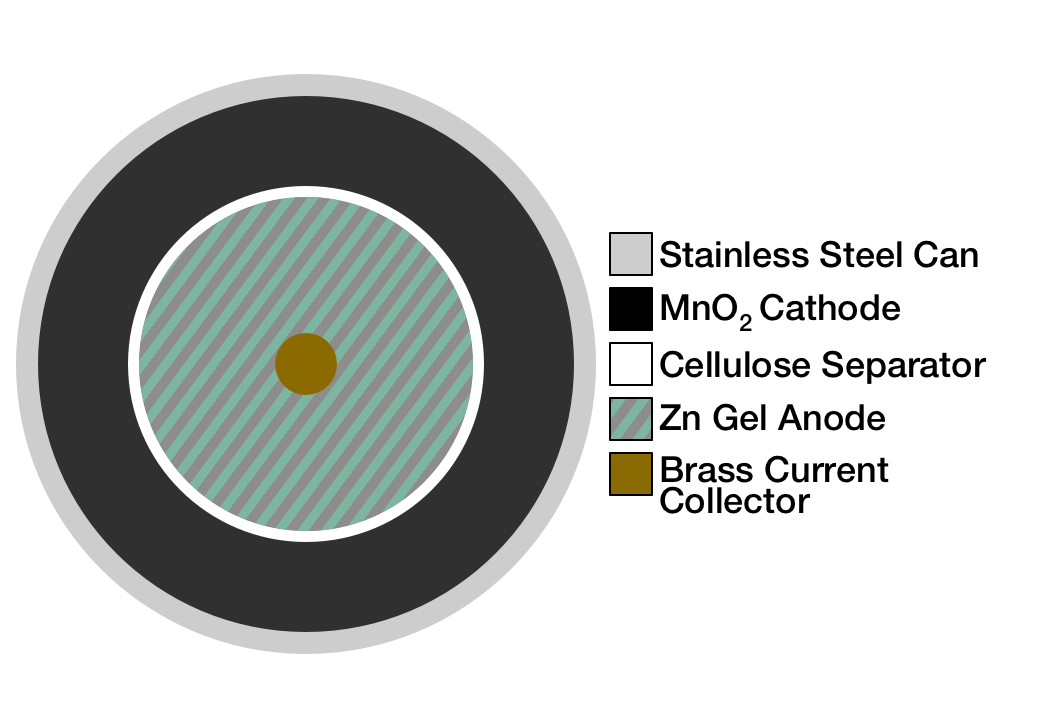
\includegraphics[width=0.80\textwidth]{ch3-dbb/Images/aaschem.png}
    \repeatcaption{fig:aaschem}{Schematic of construction of a alkaline AA battery. Components are labeled according to the legend.}
\end{figure}

\begin{table}[htb]
\centering
  \repeatcaptiont{tab:table3}{Materials properties of electrode materials in an alkaline battery}
  \begin{tabular}{*{4}{l}}
    \hline
    Material & Density (g/cm$^3$) & Bulk modulus (GPa) & Reference\\
    \hline
        Zinc (Zn)& 7.05 & 72.0 & ~\cite{Kaye2014-am}\\
        Zinc oxide (ZnO) & 5.06 & 134.0 & ~\cite{Munro2002-pg}\\
        Zn gel & 3.64 (est.) & 57.6 (est.) & ~\cite{Kaye2014-am,Murei2007-ke}\\
        Electrolytic (\ce{MnO2}) & 4.55 & 54.5 & ~\cite{Robert1990-zl,Tao2013-vg}\\
        Groutite (MnOOH) & 4.14 & 39.8 & ~\cite{Robert1990-zl,Tao2013-vg}\\
  \end{tabular}
\end{table}



\section{Experimental methods}
\label{sec:bw:exp}
\label{sec:dbb:results}

\section{Morphology characterization and coefficient of restitution evolution during discharge}
As an alkaline battery is discharged, the anode undergoes oxidation from Zn to ZnO, as seen in Eq.~\ref{eq:zn1} and~\ref{eq:zn2}, while the cathode is reduced from {\ce{MnO_2}} to MnOOH, shown in Eq.~\ref{eq:mn}.

\begin{equation}
{\ce{Zn + 4OH^- -> Zn(OH)^{2-}_{4} + 2e^-}}
\label{eq:zn1}
\end{equation}
\begin{equation}
{\ce{Zn(OH)^{2-}_{4} -> ZnO + H_{2}O + 2OH^-}}
\label{eq:zn2}
\end{equation}
\begin{equation}
{\ce{MnO_{2} + H_{2}O + e- -> MnOOH + OH^-}}
\label{eq:mn}
\end{equation}

\noindent Equation~\ref{eq:zn1} shows that the battery produces {\ce{Zn(OH)^{2-}_{4}} ions in solution until the electrolyte becomes supersaturated, at which point it begins to precipitate as ZnO ~\cite{linden}.

\textit{Post mortem} analysis shows that in alkaline AA batteries, the Zn gel anode initially exists as discrete Zn particles in a matrix of KOH electrolyte and a gelling agent. After discharge, the anode densifies into a porous ZnO solid that appears more compact closer to the separator, as shown in Fig.~\ref{fig:SEM}. The densification of the anode affects the mechanical properties of the battery. The COR, which measures the elasticity of a collision between two objects, is one such mechanical property that can be determined as shown in Eq.~\ref{eq:cor}.



\begin{figure}[htb]
  \centering
    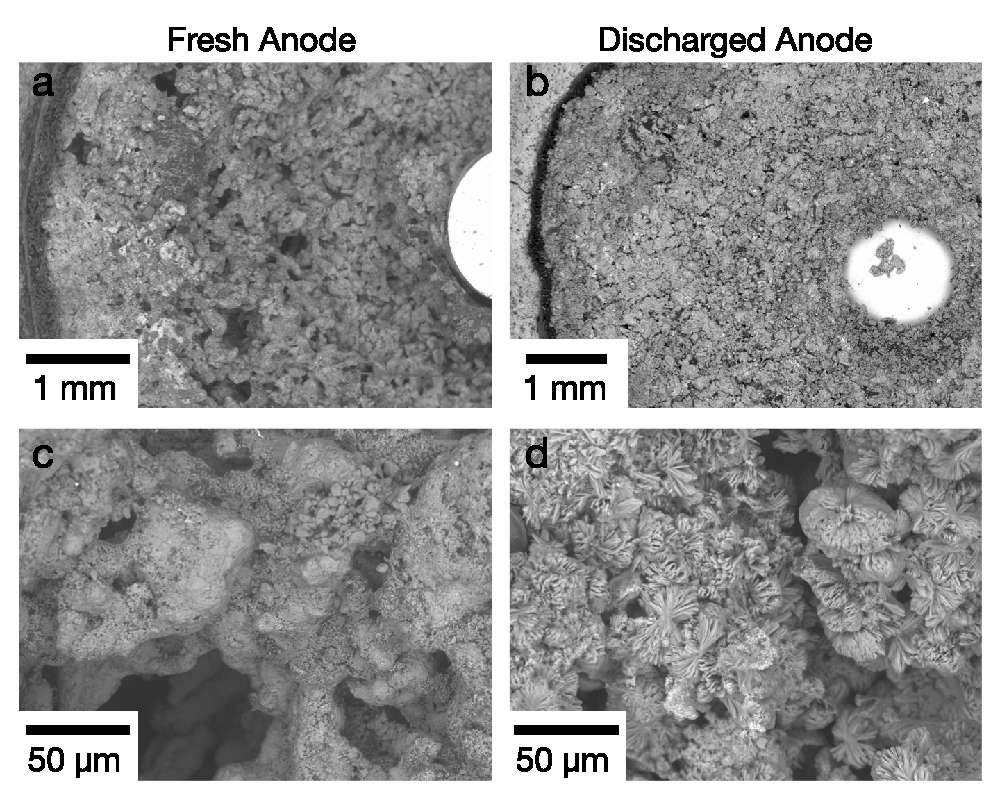
\includegraphics[width=0.8\textwidth]{ch3-dbb/Images/ZnSEM.eps}
    \caption[SEM images of sectioned fresh and fully discharged alkaline batteries]{a) SEM image of ``fresh" cell. b) SEM image of the same cell after full discharge (2850 mAh passed). c) High mag. SEM image showing fresh Zn particles. d) High mag. SEM image showing coagulated ZnO particles after full discharge.}
    \label{fig:SEM}
\end{figure}

\begin{equation}
COR = \frac{1}{N} \sum\limits_{n=1}^N \sqrt{\frac{h_{n+1}}{h_n}}
\label{eq:cor}
\end{equation}

\noindent where \(N\) is the number of bounces, and \(h\) denotes the bounce heights determined from Eq.~\ref{eq:bounce}. Using the bounce test described previously, the COR of alkaline batteries was measured through full discharge.

Figure~\ref{fig:COR1to3} shows the evolution of the COR for three identical AA cells as capacity is passed in increments of 280 milliamp-hours (mAh) at 280 mA, corresponding to a rate of C/10. The inset shows a composited image of the corresponding drop tests for a single cell. A sharp increase in COR occurs at 80\% SOC, when 560 mAh have passed, followed by asymptotic leveling of the COR at a value of 0.66\(\pm\) 0.02 after 50\% SOC (1400 mAh passed).  The three cells show excellent agreement in the low and high COR regimes, and the variance in the dynamic regime (80\% to 50\% SOC) shows that there is some variance from cell to cell in ZnO growth.

\clearpage

\begin{figure}[hbt]
  \centering
    \includegraphics[width=0.8\textwidth]{ch3-dbb/Images/cor280.pdf}
    \caption[Coefficient of restitution evolution at 280 mA.]{Coefficient of restitution as a function of capacity passed at 280 mA. Inset: Composited image of bounce behavior for a single cell over full depth of discharge}
    \label{fig:COR1to3}
\end{figure}

To show the transition between the low COR and high COR regimes more clearly and to gauge the effect of discharge rate on the COR evolution, cells were discharged at 50 mA in one hour intervals (50 mAh) prior to bounce testing, corresponding to a rate of roughly C/57. As shown in Figure~\ref{fig:50mah} the COR is constant for low depths of discharge, similar to the cells discharged at 280 mA. The rise in COR begins after 450 mAh have been passed, which is roughly 100 mAh earlier than in the cells discharged at 280 mA. The leveling of COR for these cells occurs at 950 mAh passed, which is roughly 450 mAh earlier than the saturation point for COR of cells discharged at 280 mA. It has been shown previously by Horn et al~\cite{horn} that lower discharge rates will result in a more even distribution of ZnO in the anode, compared to that of a higher discharge rate, thus a more even distribution of ZnO. We posit that because ZnO is the major contributor to the changes in mechanical properties of the battery, a more even distribution results in earlier leveling of the COR.

\begin{figure}[ht]
  \centering
    \includegraphics[width=0.8\textwidth]{ch3-dbb/Images/50mAh.eps}
    \caption[Coefficient of restitution evolution at 50 mA.]{Coefficient of restitution as a function of capacity passed at 50 mA in 50 mAh increments.}
    \label{fig:50mah}
\end{figure}


\section{Possible reasons for COR evolution}

As the stainless steel casing does not change or partake in the electrochemical reaction, four possible effects associated with discharging an alkaline battery may be correlated with the observed change in COR: 1) mass loss, 2) reduction of the cathode from {\ce{MnO_2}} to {\ce{MnOOH}}, 3) water consumption, and 4) oxidation of the anode from Zn to ZnO. We will discuss each of these possibilities in the remainder of the chapter. 

\subsection{Mass loss and cathode reduction}

Mass loss can be discounted, as under all operating conditions no change was observed in the mass of each battery. The cells are effectively sealed, but have safety valves to handle \ce{H2} generation which results from corrosion of the zinc,~\cite{linden} and again, no mass loss was measured during the experiments. 

The EDXRD spectra for the {\ce{MnO_2}} cathode shows peak shifts that begin immediately upon discharge, at least 400 mAh before the onset of COR increase, as shown in Figure~\ref{fig:mno2}. As reduction of the cathode is a linear process, it does not correlate clearly with the non-linear increase in COR.

\begin{figure}[htb]
\centering
    \includegraphics[width=0.8\textwidth]{ch3-dbb/Images/MnO2XRD.eps}
    \caption[Representative \ce{MnO2} EDXRD spectra at 100 mA discharge rate.]{Representative \ce{MnO2} EDXRD spectra at 100 mA discharge rate.}
    \label{fig:mno2}
\end{figure}

\subsection{Water consumption and ZnO formation}

Analysis of the discharge reaction and physical properties of water, Zn, and ZnO reveals that these two aspects are strongly coupled.  While the density of ZnO (5.61 g/cm\(^3\)) is less than that of Zn (7.14 g/cm\(^3\)), the density of water with 8.9 M KOH is 1.41 g/cm\(^3.\)  Complicating the system is the use of proprietary blends of gelation agents added to the anode (typically combinations of cellulose and polyethylene glycol), so we will assume a composite density of 1.40 g/cm\(^3.\)~\cite{linden}  Equations~\ref{eq:zn1},~\ref{eq:zn2}, and~\ref{eq:mn} show that for every mole of Zn eventually oxidized to ZnO, and every mole of {\ce{MnO_2}} reduced to MnOOH, one mole of \ce{H2O} must be consumed.  This means that for 2800 mAh of charge passed, 0.94 g of \ce{H2O} must be consumed between the protonation of the {\ce{MnO_2}} and the oxidation of the zinc. 

We devised the following test to determine if water removal, without ZnO conversion, caused the increase in COR:  three AA cells, one at 100\% SOC (as-received), 50\% SOC (half-discharged), and 0\% SOC (fully-discharged), were modified by removing the top 1 cm$^2$ of casing, exposing both the anode and cathode.  The COR of cell was then measured once before and again after dehydration in a vacuum oven at 25\celsius~for 72 hours.

To ensure that water was removed from the entire cell (and not just the cathode), we then ran a separate test where 1 g of zinc anode gel was removed before and after desiccation. Each sample (as received and desiccated at each state of charge) was held at 80\celsius~for 24 hours. The zinc gel, before our desiccation method, lost 0.2 $\pm$ 0.002 g when dried at 80\celsius~in vacuum. The zinc gels, after desiccation, lost negligible (lower than the scale precision) amounts of water.  This gave us confidence that water was removed through the cell during our 25\celsius~desiccation. Additionally, the non-desiccated zinc gel could be "spread" readily with a spatula; in contrast, the desiccated zinc was rigid and would crumble when enough shear was applied to move the particles. Both were notably different from the discharged zinc, which was a rigid, concrete-like mass that was difficult to break apart. 

Removing the case decreased the overall coefficient of restitution. Table~\ref{tab:cortable} indicates that there was no meaningful change in the COR when the cells at different states of charge were dehydrated at 25\celsius~for three days, despite the aforementioned water loss and "stiffening" of the anode. Thus, water removal from the cell, and particularly from the zinc gel anode, alone does not alter the COR of the cell.


\begin{table}[htb]
\centering
 \caption{\label{tab:cortable}Water content effect on coefficient of restitution.}
  \begin{tabular}{p{2.5cm}p{2.5cm}p{2.5cm}p{2.5cm}}
    \hline
    & Coefficient of restitution at 100\% SOC & Coefficient of restitution at 50\% SOC & Coefficient of restitution at 0\% SOC\\
    \hline
        As received & 0.10 $\pm$ 0.05 & 0.43 $\pm$ 0.02 & 0.43 $\pm$ 0.02\\
        Dehydrated & 0.10 $\pm$ 0.05 & 0.43 $\pm$ 0.02 & 0.42 $\pm$ 0.02\\
        Unmodified & 0.23 $\pm$ 0.02 & 0.60 $\pm$ 0.03 & 0.66 $\pm$ 0.02\\
  \end{tabular}
\end{table}

What is more likely the cause of the increased COR is is a combination of water being consumed as zinc oxide forms as indicated by reactions 1 and 2.  What we will show in subsequent sections is that while water is consumed to form zinc oxide throughout the anode, the COR change appears to correlate with the point at which ZnO is present through the thickness of the the Zn gel anode.

\section{Comparison of bounce test data to \textit{in situ} data}

\subsection{Comparison to electrochemical impedance spectroscopy data}

One method for measuring the evolution of interfaces within a battery is electrochemical impedance spectroscopy (EIS).~\cite{dornbusch,ghavami} EIS was performed after every 10\% of capacity discharged (280 mAh) to observe the effects of anode oxidation on the impedance of the battery. We found a high value for the imaginary (Z") and  real (Z') components of impedance in the as-received battery, with a two order of magnitude drop in both following 10\% discharge of the cell. This drop was most evident in the low frequency regime of the EIS spectra, often associated with mass transport limitations. We believe this high initial impedance of the cell is related to a proprietary polymeric coating on the zinc anode used in this brand of battery to improve the shelf life.  It was confirmed that while other brands of alkaline AA batteries do not have this high initial electrochemical impedance, they do exhibit the same increase in COR as a function of depth of discharge. These results, while of interest, do not give a clear indication of the cause of the increase and leveling of the COR. While not crucial to our hypothesis, a detailed discussion of the EIS model that was developed is presented along with references to established EIS models in Appendix~\ref{ch:eis}. EIS suggests that some structural evolution occurs within the anode, but a method is required to characterize discrete volumes within the battery to understand the oxidation process.  

\subsection{Comparison to EDXRD data}

Recent studies have shown that performing \textit{in situ} EDXRD on batteries during discharge can probe the evolution of the internal components.~\cite{gallaway,haibel,Manke2007-yj} Using similar methods, \textit{in situ} EDXRD was performed in AA batteries at three discharge rates: 100 mA, 200 mA, and 300 mA. The x-ray beam was incident along the width of the battery, which allows for collection of spatially resolved data, providing a measure of the oxidation of Zn to ZnO at both edges of the anode: the separator and the current collector. In all three cells, we see that ZnO forms at the separator interface (Fig.~\ref{fig:znxrd}a,c,e) before forming at the current collector interface (Fig.~\ref{fig:znxrd}b,d,f). The capacity passed at which ZnO is present at each interface is detailed in Table~\ref{tab:znotable}.

\begin{table}[htb]
\centering
  \caption{\label{tab:znotable}Formation of ZnO within the anode.}
  \begin{tabular}{*{3}{l}}
    \hline
       Discharge rate (mA)&\specialcell{Capacity passed before\\appearance of ZnO\\at separator (mAh)}&\specialcell{Capacity passed before\\appearance of ZnO\\at current collector (mAh)}\\
    \hline
        100 & 200 - 300 & 300 - 400\\
        200 & 200 - 400 & 400 - 600\\
        300 & 300 - 600 & 300 - 600\\
  \end{tabular}
\end{table}


These spectra confirm the results of Horn et al,~\cite{horn} who have shown that at higher discharge rates, ZnO will grow preferentially at the separator interface before growing through the anode towards the current collector. They have found that ZnO initially grows as a shell around the Zn particles (Type I ZnO) through solution-precipitation of {\ce{Zn(OH)^{2-}_{4}}. Once the particle is completely enveloped in Type I ZnO it begins to oxidize and deposit onto the the inside surface of the Type I ZnO shell via a second solution-precipitation step (Type II ZnO). Based on the EDXRD spectra in Fig.~\ref{fig:znxrd}, the oxidation of Zn in the cell ultimately forms a percolation network of ZnO from the separator to the current collector, and because of the axial symmetry of the cell, detection of radial percolation also suggest percolation throughout the entire cell. This agrees well with the results of Arise et al.,~\cite{arise} who have shown that following initial precipitation of ZnO onto the anode surface, the particles will coarsen and form dense films. It is also supported by the \textit{in situ} x-ray microtomography performed by Haibel et al.,~\cite{haibel}, who show that the growth front of ZnO in an alkaline cell travels from the separator to the current collecting pin as a function of depth of discharge.

\figskip{fig:znxrd}

\begin{figure}[htb]
\centering
    \includegraphics[width=\textwidth]{ch3-dbb/Images/FullZnXRD.eps}
    \caption[XRD progression of anode at separator and current collector interfaces at 100 mA, 200 mA, and 300 mA discharge rates.]{XRD progression of anode at separator and current collector interfaces at \textbf{(a,b)} 100 mA, \textbf{(c,d)} 200 mA, and \textbf{(e,f)} 300 mA discharge rates. ZnO peaks are denoted by green dashed lines, and Zn peaks are denoted by red dashed lines.}
    \label{fig:znxrd}
\end{figure}
\clearpage

Comparing the bounce test data presented in Fig.~\ref{fig:COR1to3} with the EDXRD spectra in Fig.~\ref{fig:znxrd}, it is clear that the formation of this percolation pathway occurs at the same time that the COR increases. This hypothesis is supported by the use of ZnO as an industrial additive to increase the COR of materials,~\cite{nesbitt_golf} and previous studies performed on ceramic/metal composites (cermets),~\cite{hussainova} in which increasing the ceramic content of a cermet will result in an increase in the COR, assuming the ceramic has a higher elastic modulus relative to the metal matrix. Table 3 shows relevant materials properties for the alkaline battery system. Treating the partially oxidized anode as a cermet, and knowing that the Zn to ZnO transition results in 107\% increase in bulk modulus, we expect an increase in COR as the Zn particles are oxidized.


\begin{table}[htb]
\centering
  \caption{\label{tab:table3}Materials properties of electrode materials in an alkaline battery}
  \begin{tabular}{*{4}{l}}
    \hline
    Material & Density (g/cm$^3$) & Bulk modulus (GPa) & Reference\\
    \hline
        Zinc (Zn)& 7.05 & 72.0 & ~\cite{Kaye2014-am}\\
        Zinc oxide (ZnO) & 5.06 & 134.0 & ~\cite{Munro2002-pg}\\
        Zn gel & 3.64 (est.) & 57.6 (est.) & ~\cite{Kaye2014-am,Murei2007-ke}\\
        Electrolytic (\ce{MnO2}) & 4.55 & 54.5 & ~\cite{Robert1990-zl,Tao2013-vg}\\
        Groutite (MnOOH) & 4.14 & 39.8 & ~\cite{Robert1990-zl,Tao2013-vg}\\
  \end{tabular}
\end{table}


% \begin{table}[h]
%     \centering
%         \caption{\label{tab:table3}Materials Properties}
%         \begin{tabular}{lll}
%             Material & Density (g/cm$^3$)~\cite\{EncOfMat\} & Bulk Modulus (GPa)\\
%             Zinc (Zn) & 7.05 & 59~\cite\{Ledbetter1977-rl\} \\
%             Zinc oxide (ZnO) & 5.06 & 134~\cite\{Munro2002-pg\}    \\
%             Ramsdellite (\ce\{MnO2\}) & 4.37\ & 119~\cite\{Lin2011-ur\}   \\
%             Groutite (MnOOH)          & 4.14\ & 96~\cite\{Suzuki2013-dt\}   
%         \end{tabular}
% \end{table}

The leveling of the COR is best explained using the methods of Antonyuk et al.,~\cite{antonyuk} who have found that a material's COR will saturate at the point at which it no longer yields plastically. Using Faradaic analysis, after 1400 mAh of charge is passed (50\% SOC), 1.71 g of Zn will be consumed at the anode, while 2.13 g of ZnO will be produced. At this state of charge half the Zn has been converted to ZnO, assuming a zinc limited battery, making ZnO the majority phase in the anode, both volumetrically and gravimetrically. As per Horn et al and Arise et al.,~\cite{horn,arise} the Type I ZnO shells will form together and sequester the liquid electrolyte while there is remaining free volume within the anode, while the bulk of the Zn particle will be oxidized to Type II ZnO. Initially, the anode gel consists of discrete Zn particles that can move within the gel matrix. Once percolation begins, this motion becomes suppressed. Once the anode densifies, as shown in Figure 1b, it becomes a stiff ceramic core that arrests all movement of the discrete Zn particles, and the COR levels off. This process is detailed in Fig.~\ref{fig:sketch}, which shows the initial gel, the growth of Type I ZnO, the percolation of ZnO in the anode, and the final densification of the anode.
\begin{figure}[h]
  \centering
    \includegraphics[width=0.8\textwidth]{ch3-dbb/Images/dbbsketch.eps}
    \caption[The progression of ZnO formation in the alkaline AA anode]{The progression of ZnO formation in the anode. \textbf{(a)} The initial anode gel comprised of Zn particles in an electrolyte/cellulose matrix. \textbf{(b)} Formation of Type I ZnO shells on Zn particles. c) Formation of a percolation pathway. \textbf{(d)} Densification of the anode.}
    \label{fig:sketch}
\end{figure}
\section{Conclusions}
\label{sec:alkbw:conclusion}

\chapter{Conclusion\label{ch:conclusion}}

\section{Summary}
\label{sec:conclusion:summary} % Conclusion
\section{Future Work}

-Alkaline AA cathode

-Fancy model to deconvolute data

-Custom built solution

  % Future work

\appendix % all chapters following will be labeled as appendices
\chapter{Electrochemical impedance spectroscopy and equivalent circuit model for AA alkaline batteries\label{ch:eis}}

Our results in Fig.~\ref{fig:EIS} agree with previous impedance spectroscopy experiments on alkaline LR6-type cells.~\cite{wang,root} In the Nyquist plots, high reactance (Z") and resistance (Z') are visible in the as-received cell, with a two order of magnitude drop in both following 10\% discharge of the cell. A maximum in solution resistance occurs at 50\% SOC. Reactance remains constant. Our tests of our system show that it can be modeled with a standard Randles circuit, modified by the addition of a second phase with separate charge-transfer and double-layer capacitance impedance values. This model is shown in Fig.~\ref{fig:EIS}a. Over time, the ohmic impedance of the system, typically dominated by the ionic impedance of the electrolyte, stays roughly constant with state of charge (SOC), up until 50\% SOC, when a significant spike in ohmic impedance occurs. This increase correlates with the leveling of the coefficient of restitution changes caused by the transition between the formation of Type I ZnO to Type II ZnO. The double-layer capacitance of both phases present decreases with decreasing state-of-charge. This suggests that there is a continuous decrease in the total surface area of the available Zn anode with cycling, which correlates well with the phase transformation from Zn to ZnO, as ZnO is less dense than Zn. This is in strong agreement with Haibel, Manke and Gallaway.~\cite{haibel,Manke2007-yj,gallaway}  What we see is a complex mix within the impedance data, where increasing impedance throughout the entire discharge is attributed to 1) loss of solvent (consumption of water) in the protonation of \ce{MnO_2} and the oxidation of Zn, 2) ZnO formation which passivates and blocks the Zn surface, and 3) increasing concentration of alkaline salts in the remaining water which decreases the conductivity of the electrolyte above.~\cite{linden}

\begin{figure}[htb]
  \centering
    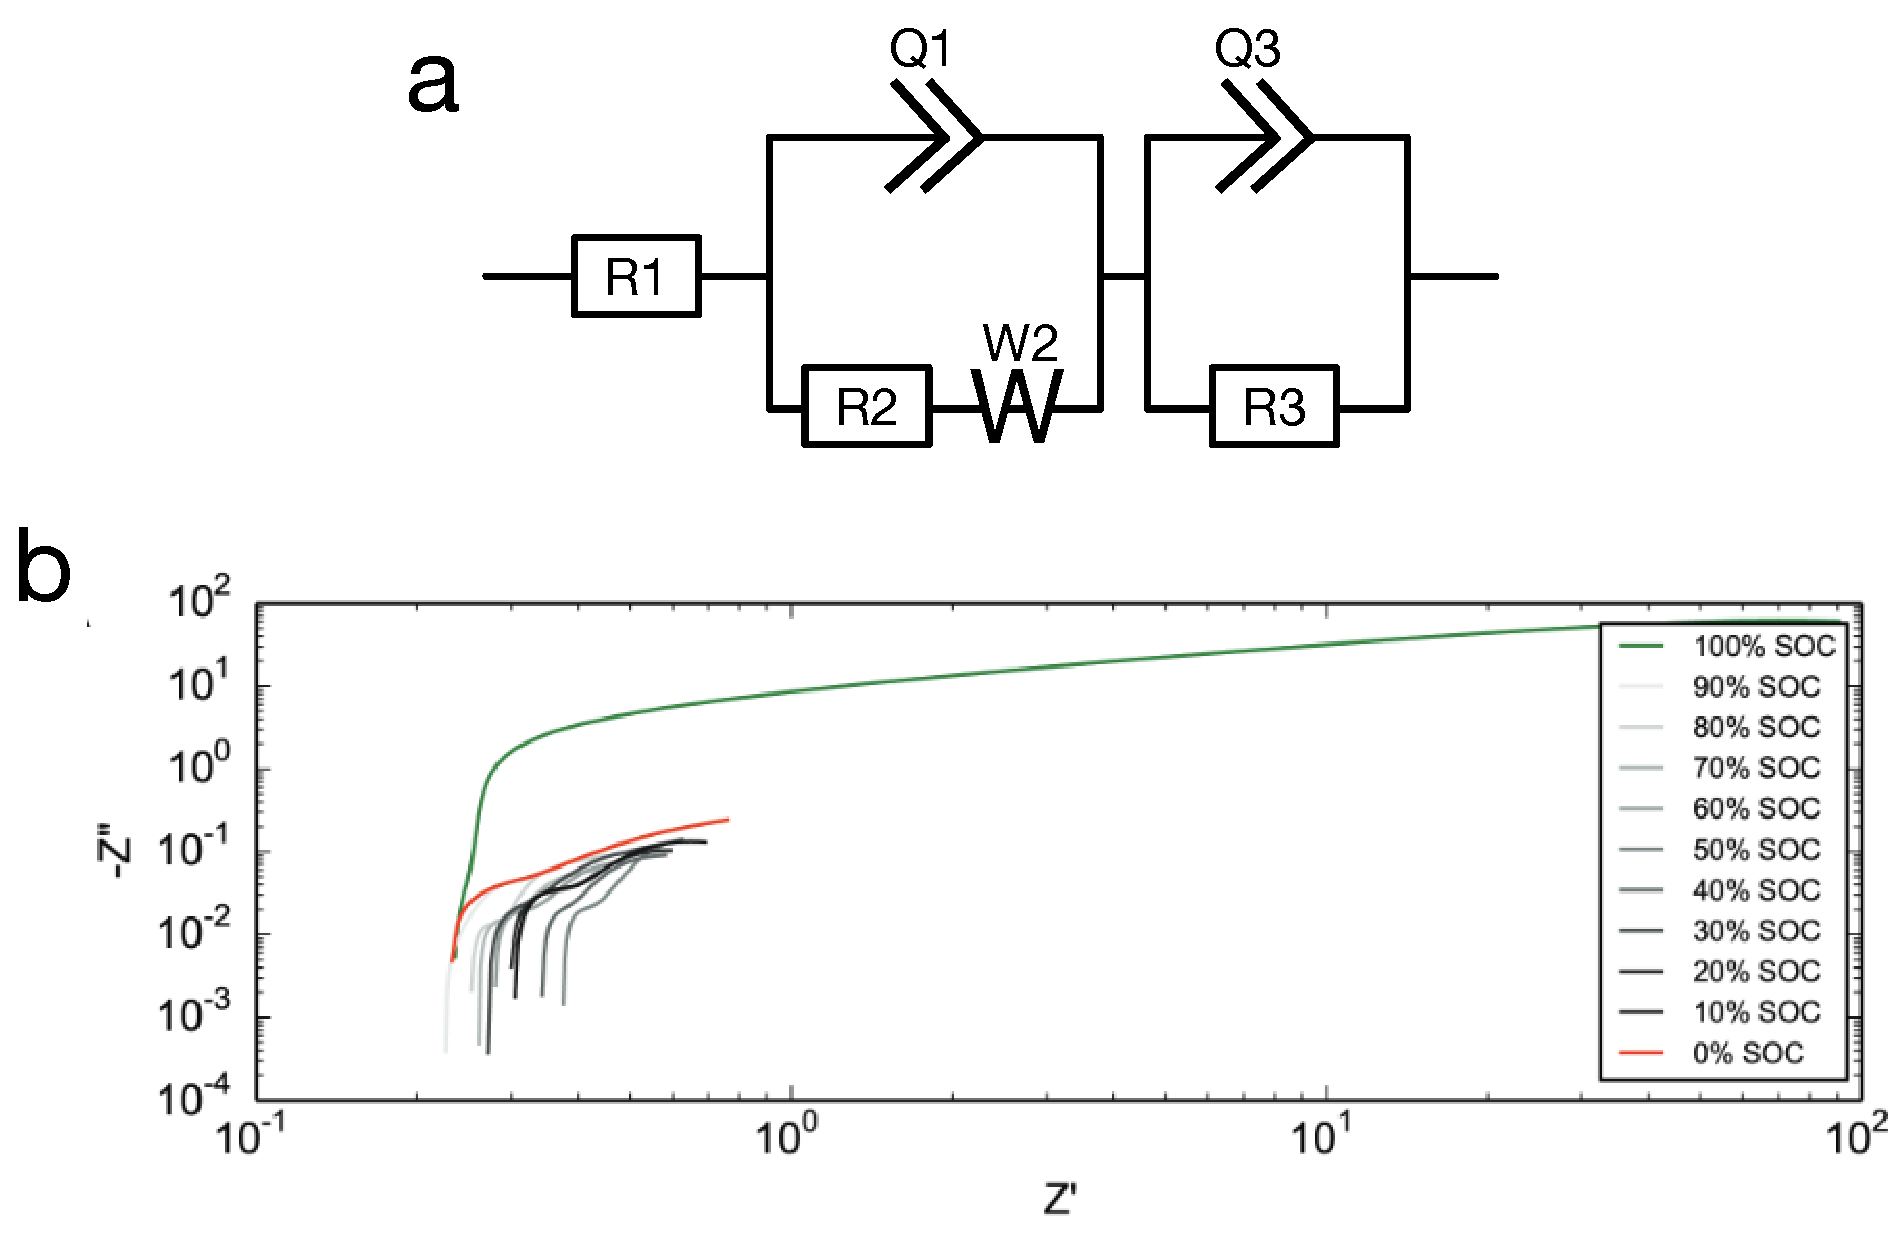
\includegraphics[width=\textwidth]{ch-appendices/images/Supp5.pdf}
    \caption[Equivalent circuit model and Nyquist plot for \textit{in situ} EIS performed on a AA alkaline battery]{a) Circuit diagram of EIS model used; b) Nyquist impedance plot for a representative cell, measured from as-received (green) to fully-discharged (red). Scans performed from 100 mHz to 100 kHz.}
    \label{fig:EIS}
\end{figure}
\chapter{Other chemistries\label{ch:otherchem}}


\chapter{Computational models and analysis methods\label{ch:comp}}

\section{Printing}

For the library copies of your dissertation, you must use archival quality printing and binding. This means acid-free paper, containing at least 25\% cotton fiber. Triangle Repocenter on Nassau Street in Princeton offers both 25\% cotton paper and 100\% cotton paper. Most people choose the 25\% cotton paper, and this is generally recommended by the binders. The 100\% copy paper is somewhat thicker and the extra expense is unnecessary. 

Triangle offers online submission of your printing and binding order at: \url{http://triangleprinceton.com/collegiatebinding/thesis/}. If you request binding from them, they will deliver the paper copies to Smith-Shattuck Bookbinding for you and allow you to pick up the completed copies at their store on Nassau Street. The whole process takes 2-3 business days, but check with them in advance during the busy thesis-printing season in April and May. 

Currently, your printed and bound dissertation copies can be single spaced. Only the electronic copy submitted to ProQuest must be double spaced. All copies must be printed single-sided, with specific margins. 

\section{Binding}

An archival-quality sewn binding is required for the library copies of your dissertation. Smith-Shattuck Bookbinding is highly recommended, and is used by most students. Triangle Repocenter will send your copies there for you, greatly simplifying the process, but you can call Smith-Shattuck with special requests. 

The ``library standard'' sewn binding is sufficient for the copies to be sent to Mudd Library. It uses a black buckram cloth cover, which is the most popular option. For extra copies for yourself and your family members, you can choose ``buckram roundback binding'', which adds decorative lines on the spine, and printing of the title and author on the front cover. For a small additional fee, you can include the Princeton University shield on the front cover and a ribbon bookmark. Leather covers are also available. See Smith-Shattuck's website for more details at: \url{http://www.thesisbookbinding.com/}. 


% Make the bibliography single spaced
\singlespacing
\bibliographystyle{unsrt}

% add the Bibliography to the Table of Contents
\cleardoublepage
\ifdefined\phantomsection
  \phantomsection  % makes hyperref recognize this section properly for pdf link
\else
\fi
\addcontentsline{toc}{chapter}{Bibliography}

% include your .bib file
\bibliography{thesis}

\end{document}

